% !TEX root = main.tex

In this paper, we present a systematic analysis of the expected performance of photometric stereo algorithms in outdoor settings. To explore the influence of these effects, we exploit the database of outdoor HDR environment maps detailed in the last section, which provides a rich sampling of the variability in outdoor illumination. To ensure the data is properly aligned temporally, only images that were captured during a continuous 6 hour time interval on each of these days, from 10:30 until 16:30, are considered. Through a theoretical analysis (inspired by \cite{sun-ivc-07}) and supported by an extensive empirical evaluation as well as a preliminary quantitative validation, we derive confidence intervals that allow us to predict when surface normals can be reconstructed more accurately and solely from the photometric cue. Instead of focusing exclusively on sun position~\cite{shen-pg-14}, our analysis incorporates the influence of all components of natural lighting: sun, sky, clouds, etc., as well as noise and surface albedo.

This paper does \emph{not} introduce a novel photometric stereo algorithm. Rather, we explore the conditions in which PS may or may not work, when faced with the challenging case of uncontrollable outdoor illumination. Our main goal is to provide guidance for future research by assessing the \emph{reconstructibility} of surface patches as a function of their orientation and the illumination conditions, given a set of HDR environment maps captured throughout a single day.

A promising approach to answer this question is to use more elaborate models of illumination---high dynamic range (HDR) environment maps~\cite{reinhard-book-05}---as input to outdoor PS. Promising results have been reported in~\cite{yu-iccp-13} for outdoor images taken within an interval of just eight hours (in a single day). However, the quality of outdoor results is reported to be inferior to that obtained in indoor environments, the decline being attributed to modest variation in sunlight. This observation leads to an interesting, yet unanswered question: had the sun path and atmosphere conditions been different on that day, could the quality of their results have been better? Or, in other words: what makes it a good day for outdoor Photometric Stereo?

%As one might expect, the answer to the question above is intrinsically tied to the orientation of a particular surface patch, the associated hemisphere of lighting directions observed by the patch, and the variation in lighting intensity in that hemisphere over the course of a day. So far, this question has only been explored in laboratory conditions or with simple directional illumination, where optimal lighting configurations can be theoretically derived~\cite{drbohlav-iccv-05,klaudiny-prl-14,shen-pg-14}. No attempt has been made at answering this question with more realistic illumination models in an outdoor setup, where lighting cannot be controlled and atmospheric effects are difficult to predict.

% Assumptions
To make this novel analysis tractable, we make the following assumptions. We consider Lambertian surface patches, and assume that at most one day of data can be used. We also assume that the dominant part of the light comes from the sky hemisphere (sun, sky, clouds, etc.) and surface patches are independent (cast shadows and inter-reflections are not modeled).

Although previous work have presented sensitivity analyses for standard PS with point light sources (\eg,~\cite{sun-ivc-07,jiang-bunke-sp-91,klaudiny-prl-14,shen-pg-14}), so far as we know, the case of outdoor PS with more complex illumination models has received little attention.

\subsubsection{Image formation model}
\label{iccp15:ifm}

Consider a small, Lambertian surface patch with normal vector ${\bf n}$ and albedo $\rho$ (w.l.o.g., assume albedo is monochromatic). At time $t$, this surface patch is observed under natural, outdoor illumination represented by the environment map $L_t(\boldomega)$ (\eg, fig.~\ref{fig:database}), with $\boldomega$ denoting a direction in the unit sphere. With an orthographic camera model, this patch is depicted as an image pixel with intensity
%
\begin{equation}
    b_t = \frac{\rho}{\pi} \int_{\Omega_{\bf n}} L_t(\mathbf{\boldomega}) \langle \boldomega, {\bf n} \rangle d\omega \,,
    \label{eqn:imageformation-continuous}
\end{equation}
%
where $\langle \cdot, \cdot \rangle$ denotes the dot product. Integration is carried out over the hemisphere of incoming light, $\Omega_{\bf n}$, defined by the local orientation ${\bf n}$ of the surface, fig.~\ref{fig:normal-diagram}. This hemisphere corresponds to an occlusion (or attached shadow) mask; only half of the pixels in the environment map contribute to the illumination of the surface patch. To make the analysis tractable and independent on object geometry, this paper focuses on the simpler case without cast shadows.

\begin{figure}
    \centering
    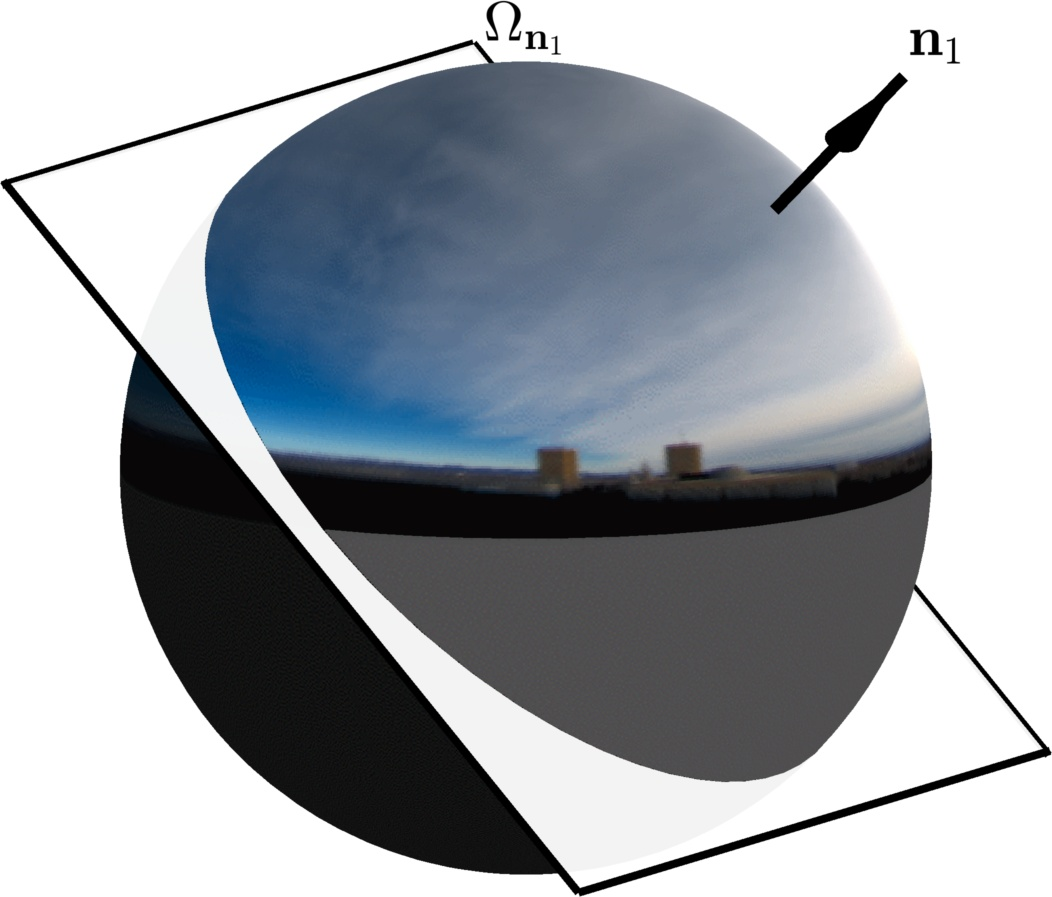
\includegraphics[width=.495\linewidth]{./figures/diagramFig/diagram1.jpg}
    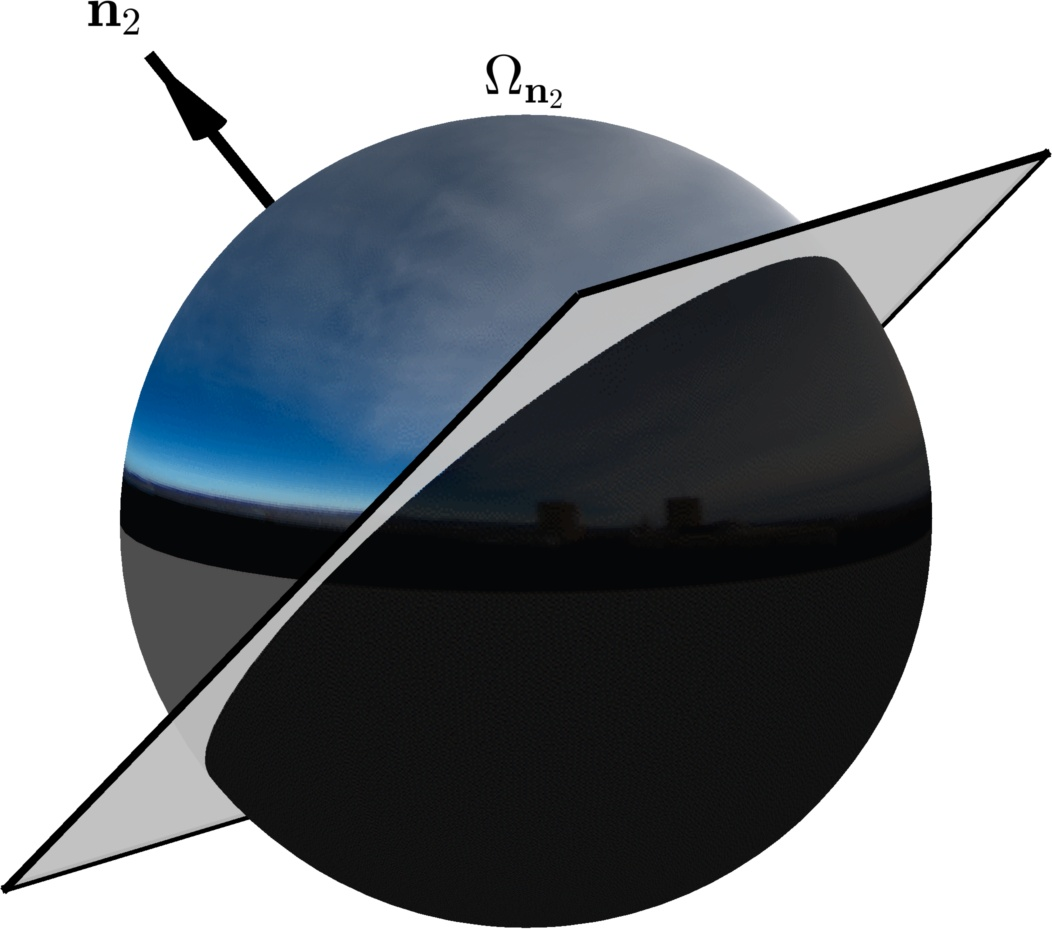
\includegraphics[width=.495\linewidth]{./figures/diagramFig/diagram2.jpg}
    \caption{A normal $\mathbf{n}$ defines an integration domain $\Omega_{\mathbf{n}}$ equivalent to a hemisphere on the entire spherical environment map. Only light emanating from this hemisphere contribute to the shading on that patch. Therefore, patches with different normals are lit differently even if the environment map is the same.}
    \label{fig:normal-diagram}
\end{figure}

This image formation model is then discretized as,
%
\begin{equation}
b_t = \frac{\rho}{\pi}\sum_{\boldomega_j \in \Omega_{\bf n}} \widehat{L}_t(\boldomega_j) \langle \boldomega_j, {\bf n} \rangle\,,
\label{eqn:imageformation-discrete}
\end{equation}
%
with $\widehat{L}_t(\boldomega_j) = L_t(\boldomega_j)\Delta\omega_j$ representing the environment map weighted by the solid angle $\Delta\omega_j$ spanned by pixel $j$ ($\Delta\omega_j$, $\forall j$, are normalized as to sum to $2\pi$). Eq.~$\eqref{eqn:imageformation-discrete}$ can be further summarized into the equivalent form
%
\begin{equation}
b_t = {\bf \bar l}_t^T \mathbf{x}
\label{eqn:imageformation-simplified}
\end{equation}
where ${\bf x} = \rho {\bf n}$ is the albedo-scaled normal vector and
\begin{equation}
{\bf \bar l}_t = \frac{1}{\pi} \sum_{\boldomega_j \in \Omega_{\bf n}} \widehat{L}_t(\boldomega_j) \boldomega_j \in \mathbb{R}^3
\label{eqn:mean-light}
\end{equation}
is interpreted as the {\em mean light vector} for the environment map at a time $t$.

Given multiple images taken at times $t \in \{1,2,\ldots,T\}$, we collect all photometric constraints for patch ${\bf x}$ to obtain:
\begin{equation}
\mathbf{b} =
\begin{bmatrix}
 b_1 \\ b_2 \\ \vdots \\ b_T
\end{bmatrix}
=
\begin{bmatrix}
 {\bf \bar l}_1^T \\ {\bf \bar l}_2^T \\ \vdots \\ {\bf \bar l}_T^T
\end{bmatrix}
{\bf x} = \mathbf{L} \mathbf{x} \,.
\label{eqn:matrix-form}
\end{equation}
With~\eqref{eqn:matrix-form}, this model of natural environmental illumination becomes quite similar to a model with a distant point light source, the well-known case in PS. However, note that each ${\bf \bar l}_t$ in ${\bf L}$ is a function of $\Omega_{\bf n}$ and, thus, of ${\bf n}$.

Most importantly, in outdoor PS, a well-defined solution ${\bf x}$ may exist even if the relative sun motion is nearly planar during a certain time interval. Instead of relying solely on sun direction, now, the solution requires non-coplanar mean light vectors ${\bf \bar l}_t$, which are determined by a comprehensive set of natural illumination factors.

\subsubsection{Modeling uncertainty}

From~\eqref{eqn:matrix-form}, the least-squares solution ${\bf x} = ({\bf L}^T{\bf L})^{-1}{\bf L}^T{\bf b}$ of outdoor PS is clearly affected by the condition number of ${\bf L}$. Thus, we next characterize how well the solution ${\bf x}$ is constrained by natural, outdoor illumination within a given time interval (\eg, one day)---which is encoded by the set of mean light vectors ${\bf \bar l}_t$ in ${\bf L}$ or, equivalently, the set of environment maps $L_t(\cdot)$.

To assess the reliability of a solution ${\bf x}$, we follow standard practice in PS~\cite{klaudiny-prl-14,sun-ivc-07} and consider image measurements corrupted by zero-mean Gaussian noise with equal variance $\sigma^2$ (as least squares estimation is only optimal for this practical, most common noise model). Thus, ${\bf b}$ in~\eqref{eqn:matrix-form} follows a normal distribution:
%
\begin{equation}
{\bf b} \sim \mathcal{N}\left( \boldmu_b, \sigma^2 {\bf I} \right)\,,
\end{equation}
%
where $\boldmu_b$ has the (unknown) uncorrupted pixel values.

Since the desired least-squares solution for the albedo-scaled normal, ${\bf x} = \left({\bf L}^T{\bf L}\right)^{-1}{\bf L}^T{\bf b}$, is a linear transformation of a Gaussian random vector, it is easy to show that
%
\begin{equation}
{\bf x} \sim \mathcal{N} \left( \boldmu_x, \sigma^2({\bf L}^T{\bf L})^{-1} \right)\,,
\end{equation}
where $\boldmu_x = \left({\bf L}^T{\bf L}\right)^{-1}{\bf L}^T\boldmu_b$ is the expected value of ${\bf x}$.
Once the albedo of a surface patch is known, we analyze its contribution to the uncertainty in the estimated normal vector, ${\bf n} = \rho^{-1}{\bf x}$, using a similar distribution,
%
\begin{equation}
{\bf n} \sim \mathcal{N} \left( \frac{\boldmu_x}{\rho}, \frac{\sigma^2}{\rho^2}({\bf L}^T{\bf L})^{-1} \right)\,.
\label{eqn:normal-distrib}
\end{equation}

The marginal distributions in~\eqref{eqn:normal-distrib} allow us to derive confidence intervals that indicate the uncertainty in each component of the least squares estimate ${\bf \hat n} = [ \hat n_x \ \hat n_y \ \hat n_z ]^T$ of ${\bf n} = [ n_x \ n_y \ n_z ]^T$. The corresponding $95\%$ confidence interval~\cite{hastie-book-09} is given by
%
\begin{equation}
\hat{\mathbf{n}} \pm \bolddelta \,, \quad \text{with } \delta_k = 1.96 \frac{\sigma\lambda_k}{\rho} \,,
\label{eqn:confidence-xyz}
\end{equation}
%
where $\lambda_k$ is the square root of the $k$th element on the diagonal of $({\bf L}^T{\bf L})^{-1}$. As expected, the sensor-dependent noise level $\sigma$ is not the only factor that determines uncertainty. The gain factor $\lambda_k/\rho$ in \eqref{eqn:confidence-xyz} reveals how outdoor illumination (the conditioning of ${\bf L}$) and albedo can amplify the effect of noise on the solution ${\bf \hat n}$. The lower the albedo $\rho$ is, the larger is the variance in the obtained estimate $\bf \hat n$ (as less light is reflected towards the camera). Our goal is then to answer the remaining question: how do natural changes in outdoor illumination affect this gain factor ($\lambda_k$) and, therefore, uncertainty?

\subsubsection{An intuitive measure of uncertainty}
\label{subsec:measure_uncertainty}

To provide a measure of uncertainty that is more intuitive than~\eqref{eqn:confidence-xyz}, we consider angular distances in degrees,
%
\begin{equation}
\theta^\pm = \cos^{-1}(\mathbf{n}^T{\bf \hat n}^\pm)\,,
\quad \text{where }
{\bf \hat n}^\pm = \frac{{\bf \hat n} \pm \bolddelta}{\lVert{\bf \hat n} \pm \bolddelta \rVert}\,.
\label{eqn:angular-dist}
\end{equation}
%
The uncertainty in the estimate of ${\bf n}$ is then summarized in a single confidence interval, in degrees,
%
\begin{equation}
\mathcal{C}_{\bf n} = [ \ 0, \ \max (\theta^\pm) \ ]\,,
\label{eqn:confidence-degrees}
\end{equation}
which indicates the expected accuracy of the estimated surface orientation ${\bf \hat n}$.

Note that the condition number, determinant, and trace of matrix $(\mathbf{L}^T\mathbf{L})^{-1}$ can also be used as measures of total variance in the estimated solutions---as done in~\cite{sun-ivc-07}---to find the optimal location of point light sources in PS. These measures are closely related to the rank of matrix $\mathbf{L}$, which must be three for a solution to exist; that is, $\mathbf{L}^T\mathbf{L}$ must be nonsingular. In practice, this matrix is always full-rank, although it is often poorly conditioned~\cite{shen-pg-14}. In the remaining sections, we consider confidence intervals $\mathcal{C}_{\bf n}$ in degrees, as they provide a more intuitive measure of uncertainty in the obtained solutions. Finally, in~\eqref{eqn:angular-dist}, the normalization of ${\bf \hat n}^\pm$ to unit length reflects the fact that part of the estimation error is propagated to the estimated albedo $\rho$ (\ie, the length of the computed least-squares solution vector ${\bf x}$). In this paper, we focus on analyzing our ability to recover geometry and will assume that the albedo is constant and known.

\subsection{Analyzing the outdoor lighting dataset}
\label{sec:iccp15-datasetanalysis}

% context, need, task, object, conclusions, perspective
Now that we are equipped with a tool to characterize the stability of surface normal estimation in outdoor PS, we proceed to apply it to all 23 days from our dataset (sec.~\ref{sec:hdrdb}) in order to determine the conditions in which surface normals can accurately be reconstructed. We first describe how the confidence intervals $\mathcal{C}_{\bf n}$ are computed and visualized, then analyze the effect of two important characteristics of outdoor lighting: the degree of cloud coverage in sec.~\ref{sec:cloud-cover-results}, and the sun elevation in sec.~\ref{sec:sun-elevation-results}.

\begin{figure}[t]
    \centering
    \begin{minipage}{.5\linewidth}
    \begin{sideways}\begin{minipage}{.4\linewidth}\centering \scriptsize 08/24/2013 \\ 85\% sun visibility \vspace{5pt} \end{minipage}\end{sideways}
    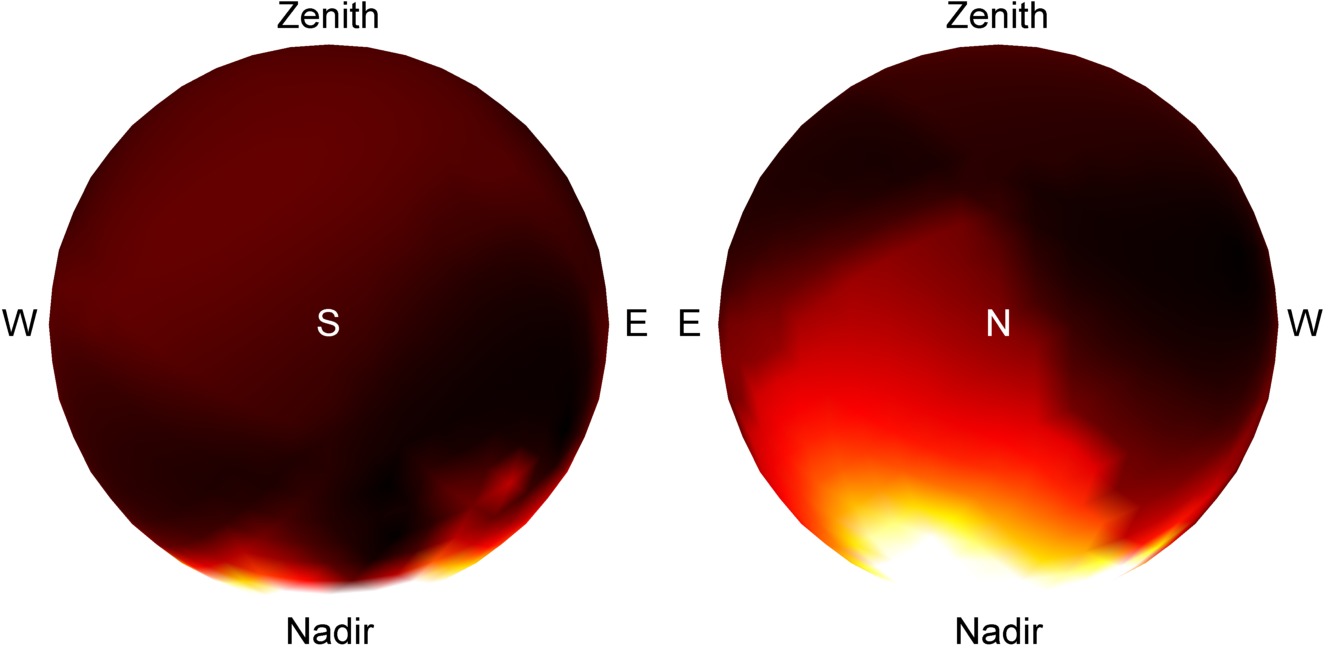
\includegraphics[width=.9\linewidth]{./figures/confidenceIntervals/20130824_10pm.png} \\
    \vspace{-.8em} \noindent\rule{\linewidth}{0.1pt}
    \begin{sideways}\begin{minipage}{.4\linewidth}\centering \scriptsize 11/06/2013 \\ 41\% sun visibility \vspace{5pt} \end{minipage}\end{sideways}
    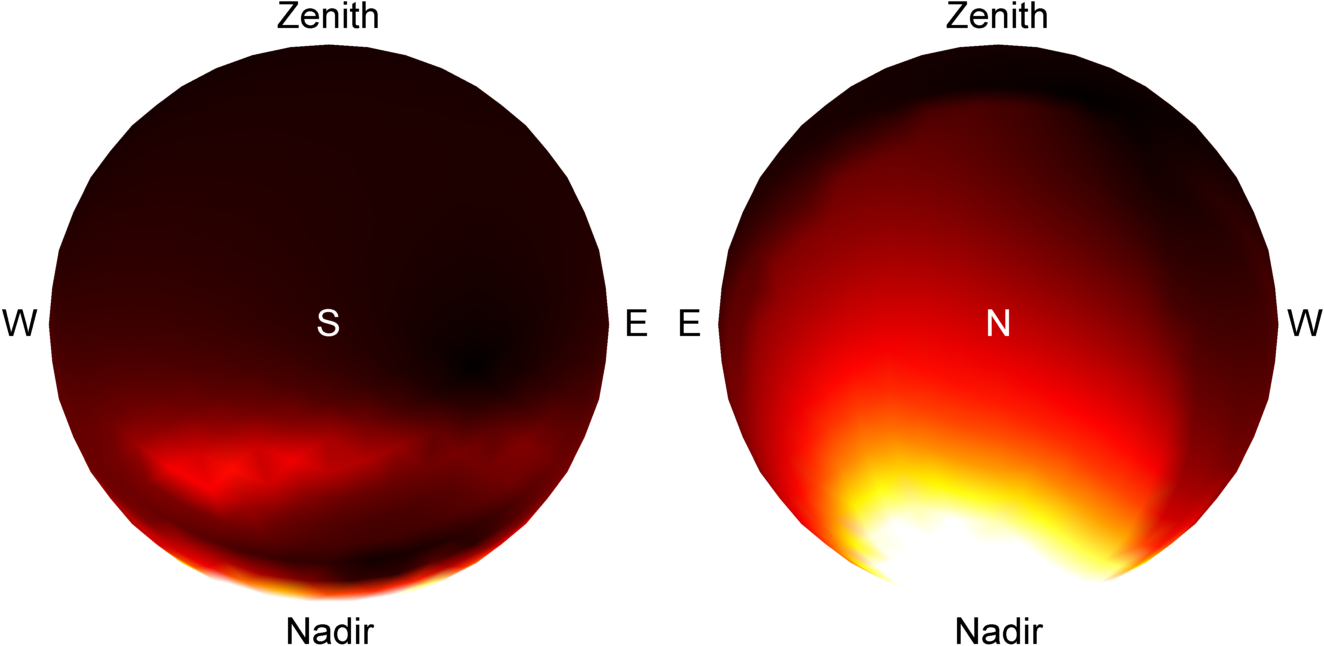
\includegraphics[width=.9\linewidth]{./figures/confidenceIntervals/20131106_10pm.png} \\
    \vspace{-.8em} \noindent\rule{\linewidth}{0.1pt}
    \begin{sideways}\begin{minipage}{.4\linewidth}\centering \scriptsize 11/08/2014 \\ 16\% sun visibility \vspace{5pt} \end{minipage}\end{sideways}
    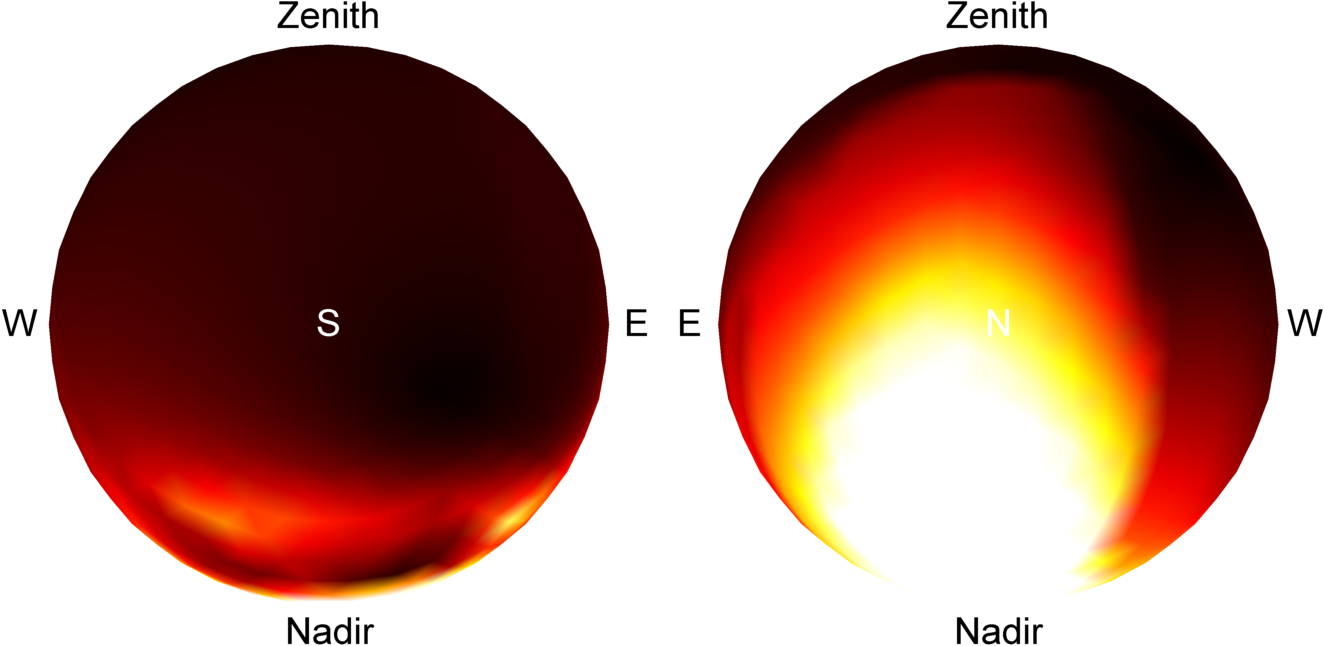
\includegraphics[width=.9\linewidth]{./figures/confidenceIntervals/20141108_10pm.png} \\
    \end{minipage}
    \vspace{3mm}
    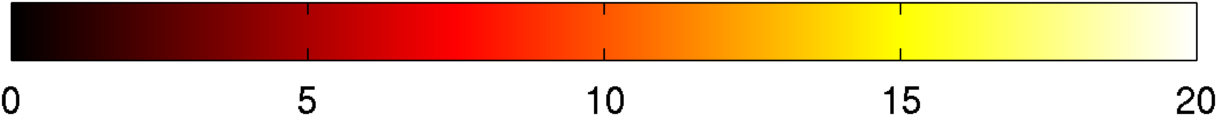
\includegraphics[width=.51\linewidth]{./figures/confidenceIntervals/colorbar.png}
    \caption{Uncertainty in normal estimation with $\sigma=1\%$ is indicated by 95\% confidence intervals (in degrees), as a function of ground-truth surface normal. Results are shown for three different days in our dataset (same days as in fig.~\ref{fig:database}). The plots show the full sphere of normals from two different viewpoints: South (left), and North (right). Cardinal directions are shown for reference. The color-coding is indicated below the plots. See companion video for an animated version of these plots.}
    \label{fig:confidence-intervals}
\end{figure}

\begin{figure*}[t]
    \centering
    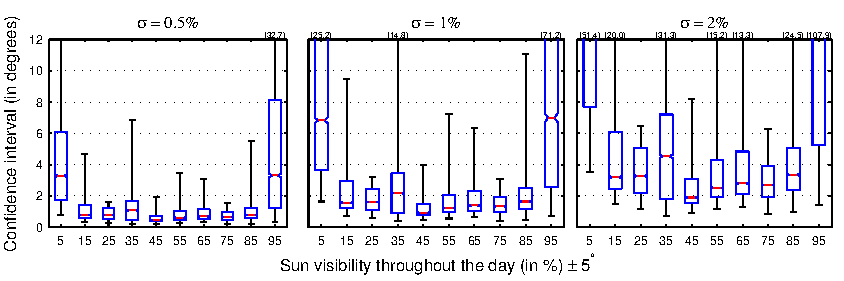
\includegraphics[width=.99\linewidth]{./figures/confidenceIntervals/sunVisibilityPlot-topHemisphere.pdf}
    \vspace{-2mm}
    \caption{Median confidence interval of normal estimates (red line) as a function of mean sun visibility over the course of the day for various values of $\sigma$. Our analysis predicts that normal reconstruction errors will likely be high if the sky is completely overcast (low sun visibility), or completely clear (high sun visibility). Good results can thus be expected in partially cloudy conditions, as shown in fig.~\ref{fig:cloud-cover}. The lower (upper) edge of each blue box indicates the 25th (75th) percentile. Statistics are computed only on normals pointing upwards to lessen ground effects.}
    \label{fig:cloud-cover-plot}
\end{figure*}


\subsubsection{Computing the stability of outdoor PS}
\label{iccp-computingstability}

We aim to apply the stability analysis of sec.~\ref{sec:analysis} on all 23 days from our dataset, and on all possible normal directions. To do so, we consider each day independently, and first sample directions on the sphere by subdividing an icosahedron three times, yielding a set of 642 potential orientations $\mathcal{N} = \{\mathbf{n}_1, ..., \mathbf{n}_{642} \}$. Then, for each $\mathbf{n}_j \in \mathcal{N}$, we build the illumination matrix $\mathbf{L}$ in~\eqref{eqn:matrix-form}, given all 6 hours of data for that day. Finally, the 95\% confidence interval $\mathcal{C}_{\mathbf{n}_j}$ is computed using~\eqref{eqn:confidence-degrees}, indicating the uncertainty (possible reconstruction error) for that normal---the higher the interval, the less stable the solution.

To compute $\mathcal{C}_{\mathbf{n}_j}$, values for the noise level $\sigma$ and the surface albedo $\rho$ from \eqref{eqn:confidence-xyz} must be chosen. For the albedo, we will consider the best case with $\rho=1$. To set $\sigma$, we first render noise-less pixel values $\mathbf{b}_j$ using the (ground-truth) normal ${\bf n}_j$ and~\eqref{eqn:matrix-form}, with ${\bf L}$ including our entire collection of environment maps. All figures have been generated with $\sigma$ set at $1\%$ of the 95th percentile value of the resulting $\mathbf{b}_j$, unless otherwise stated. This particular value is chosen to yield a small, yet non-negligible, level of noise that is similar to that in previous work~\cite{klaudiny-prl-14}. The values of $\rho$ and $\sigma$ are kept constant in order to focus solely on the influence of lighting conditions, but could be set to match particular experimental conditions if needed.

Fig.~\ref{fig:confidence-intervals} shows the result of such an analysis on the three days of fig.~\ref{fig:database}. For each day, two sides of the sphere of normal directions are shown: seen from the South (left), and from the North (right). The spheres are color-coded according to the confidence interval $\mathcal{C}_\mathbf{n}$ for each normal direction. Note that vertex interpolation is used to display full spheres, but valid data is available only at vertices (thus the staircase effect in some plots).

At first glance, we notice that normals pointing down (towards Nadir) consistently have high confidence intervals, irrespective of the illumination conditions. The stability of outdoor PS on these normals is thus expected to be low. This behavior concords with expectation: normals pointing down define integration domains $\Omega_{\mathbf{n}}$ (see fig.~\ref{fig:normal-diagram}) which mostly include the ground, whose intensity does not vary spatially throughout the day. Another interesting observation from fig.~\ref{fig:confidence-intervals} is that the same normal exhibits different confidence intervals depending on the day. This raises the question: what is the relation between outdoor illumination conditions and uncertainty in the recovered surface normal?


\subsubsection{Influence of cloud cover}
\label{sec:cloud-cover-results}

It is already apparent from fig.~\ref{fig:confidence-intervals} that cloud coverage has an effect on the uncertainty of normal reconstruction, since an overcast day (last row) clearly does not behave the same way as a day with light clouds (top row). Here, we present a more systematic analysis of the influence of cloud coverage. To control for the effect of the sun elevation (which will be explored in sec.~\ref{sec:sun-elevation-results}), the analysis is performed on days with similar sun elevations by keeping only the skies captured in October and November.

We approximate cloud coverage by computing the fraction of time that the sun is visible, \ie, that it fully shines on the scene, for a given day. To do so, we simply find the brightest spot in a sky image, and determine that the sun shines on the scene if the intensity of the brightest pixel is greater than $20\%$ of the maximum sun intensity---we determined empirically that this is the point at which the sun is bright enough to start creating cast shadows. Cloud coverage is represented by computing the mean sun visibility for a given day. A value of less than 10--15\% would indicate a mostly overcast sky, while skies are mostly clear with values above 85--90\%.

\begin{figure}[t]
    \centering
    \begin{minipage}{.5\linewidth}
    \begin{sideways}\begin{minipage}{.4\linewidth}\centering \scriptsize Clear (85-100\%)\vspace{5pt} \end{minipage}\end{sideways}
    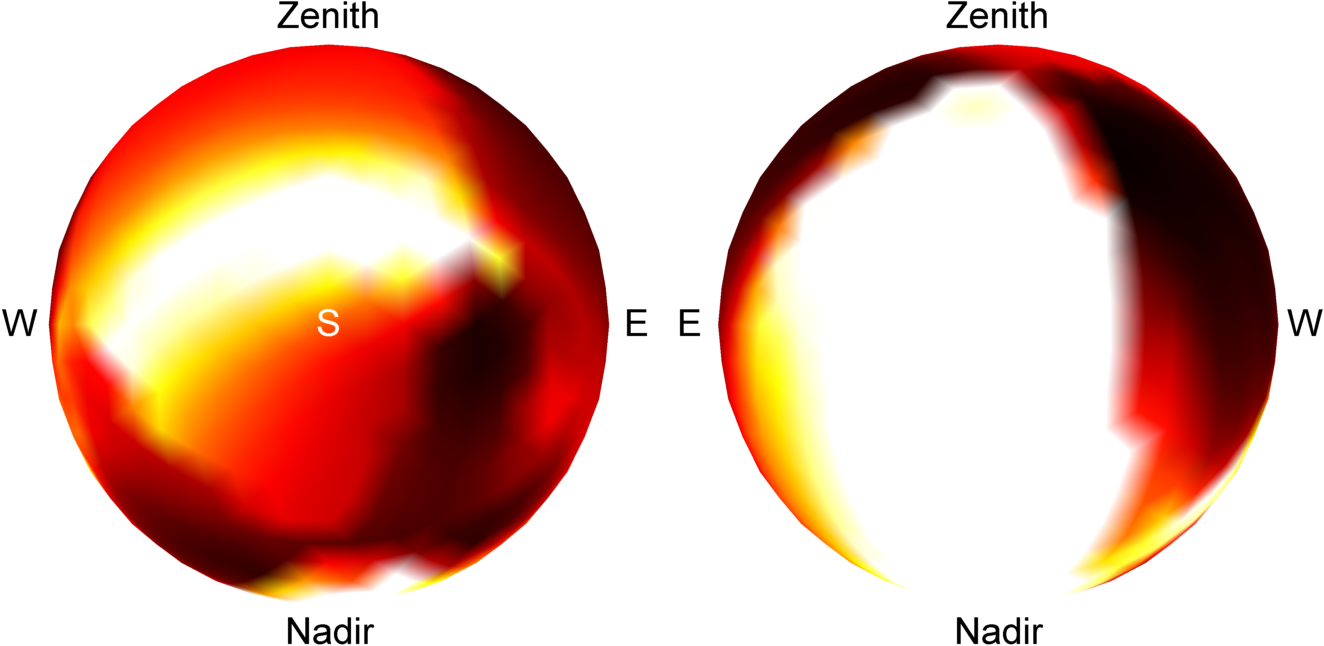
\includegraphics[width=.9\linewidth]{./figures/confidenceIntervals/clear-mean_10pm.png} \\
    \vspace{.4em} \noindent\rule{\linewidth}{0.1pt} \vspace{-.8em}
    \begin{sideways}\begin{minipage}{.4\linewidth}\centering \scriptsize Mixed Clear (50-85\%)\vspace{5pt} \end{minipage}\end{sideways}
    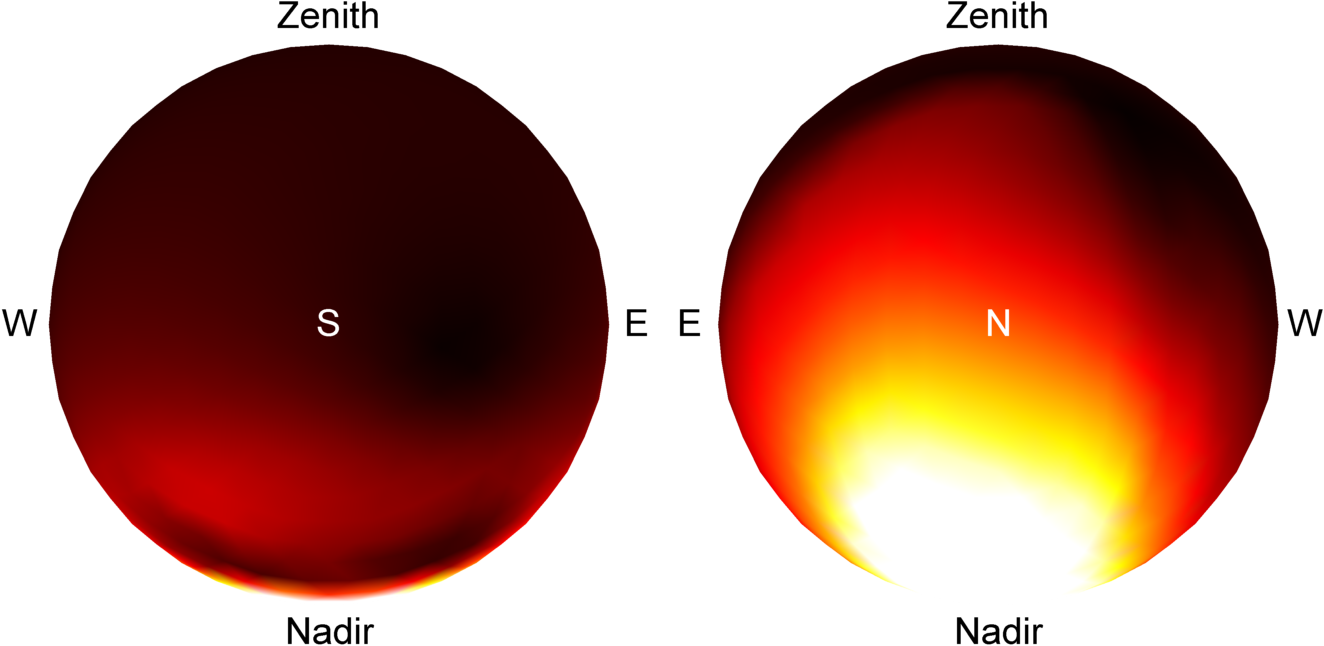
\includegraphics[width=.9\linewidth]{./figures/confidenceIntervals/mixed-clear-mean_10pm.png} \\
    \vspace{.4em} \noindent\rule{\linewidth}{0.1pt} \vspace{-.8em}
    \begin{sideways}\begin{minipage}{.4\linewidth}\centering \scriptsize Mixed Overcast (15-50\%)\vspace{5pt} \end{minipage}\end{sideways}
    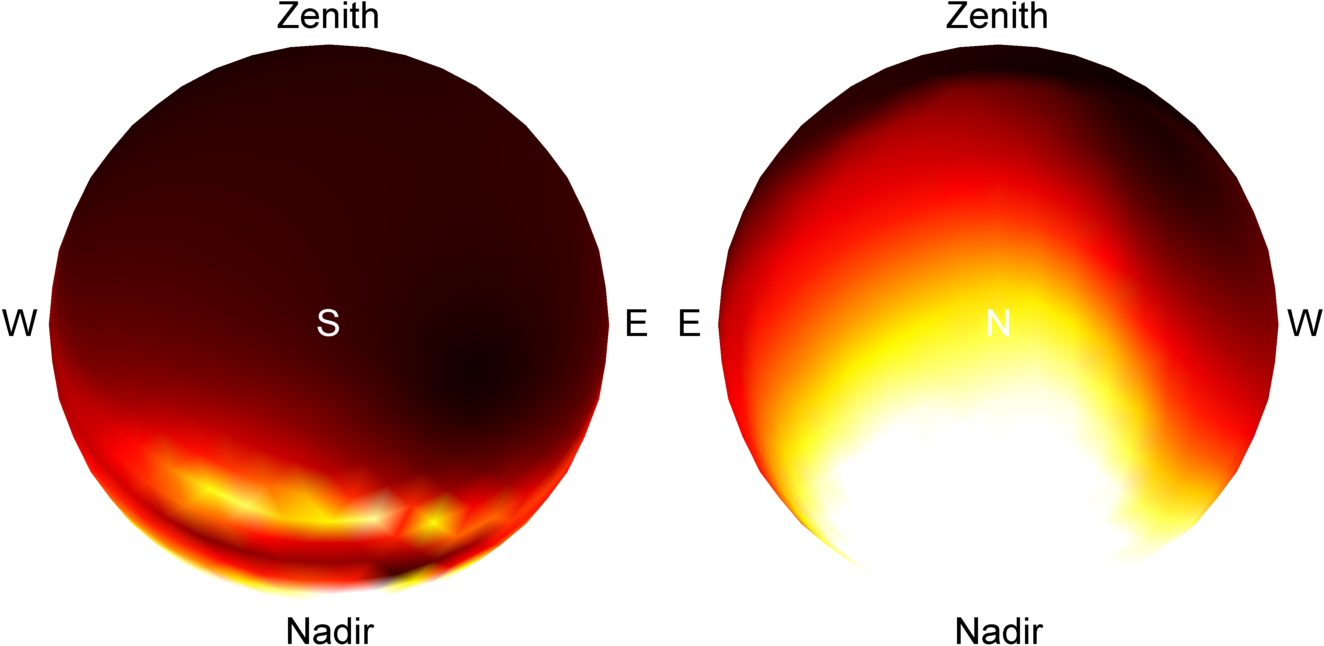
\includegraphics[width=.9\linewidth]{./figures/confidenceIntervals/mixed-overcast-mean_10pm.png} \\
    \vspace{.4em} \noindent\rule{\linewidth}{0.1pt} \vspace{-.8em}
    \begin{sideways}\begin{minipage}{.4\linewidth}\centering \scriptsize Overcast (0-15\%)\vspace{5pt} \end{minipage}\end{sideways}
    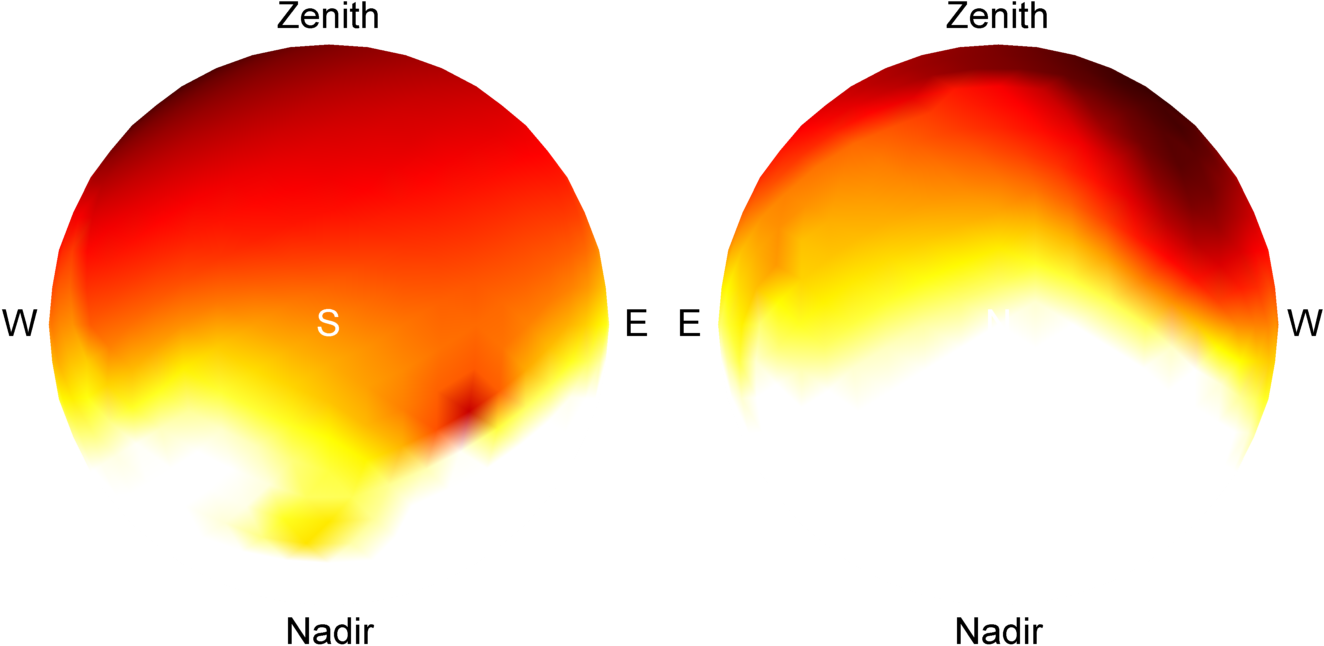
\includegraphics[width=.9\linewidth]{./figures/confidenceIntervals/overcast-mean_10pm.png} \\
    \end{minipage}
    \vspace{3mm}
    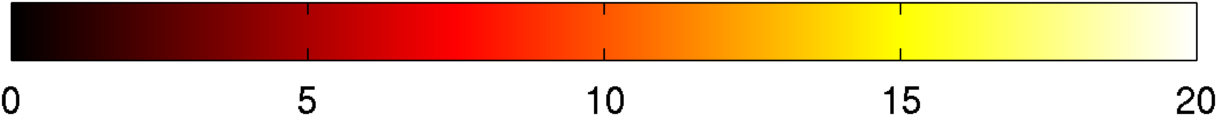
\includegraphics[width=.51\linewidth]{./figures/confidenceIntervals/colorbar.png}
    \caption{Influence of cloud cover on the 95\% confidence intervals with $\sigma=1\%$. Each row shows a different type of sky, based on sun visibility. For example, the top row shows confidence intervals averaged over all days with direct sun visibility in the range 85\%-100\%. The averaged days presented similar sun elevations. As with fig.~\ref{fig:confidence-intervals}, the plots show the full sphere of normals from two different viewpoints: South (left), and North (right).}
    \label{fig:cloud-cover}
\end{figure}

The relation between sun visibility and the confidence interval $\mathcal{C}_\mathbf{n}$ is shown in fig.~\ref{fig:cloud-cover-plot}. Normal reconstruction errors will likely be quite high in two situations: when the sky is completely overcast (low sun visibility), or completely clear (high sun visibility). Interestingly, good reconstruction results are expected for a wide range of cloud coverage conditions, ranging from 10--90\% mean sun visibility.

These results are corroborated by fig.~\ref{fig:cloud-cover}, which shows the confidence intervals themselves on a plot similar to fig.~\ref{fig:confidence-intervals}. Results there are presented by averaging the intervals of skies belonging to four groups: overcast (0--15\%), mixed overcast (15--50\%), mixed clear (50--85\%), and clear (85--100\%) days. Again, high uncertainty results are visible for the two extreme cases of fully overcast and fully clear days, while the remainder indicate more stable solutions.

% TODO: add figure to illustrate this (maybe)?
The improved conditioning in mixed skies is explained by the following key observation: cloud cover shifts the mean light vectors ${\bf \bar l}_t$ towards zenith and away from sun trajectory in the sky. Therefore, even when the sun moves along a trajectory that nearly lies on a 3D plane, as shown in fig.~\ref{fig:mlv}, cloud cover effectively causes an {\em out-of-plane} shift of the mean light vectors, making reconstruction possible.

\begin{figure}
    \centering
    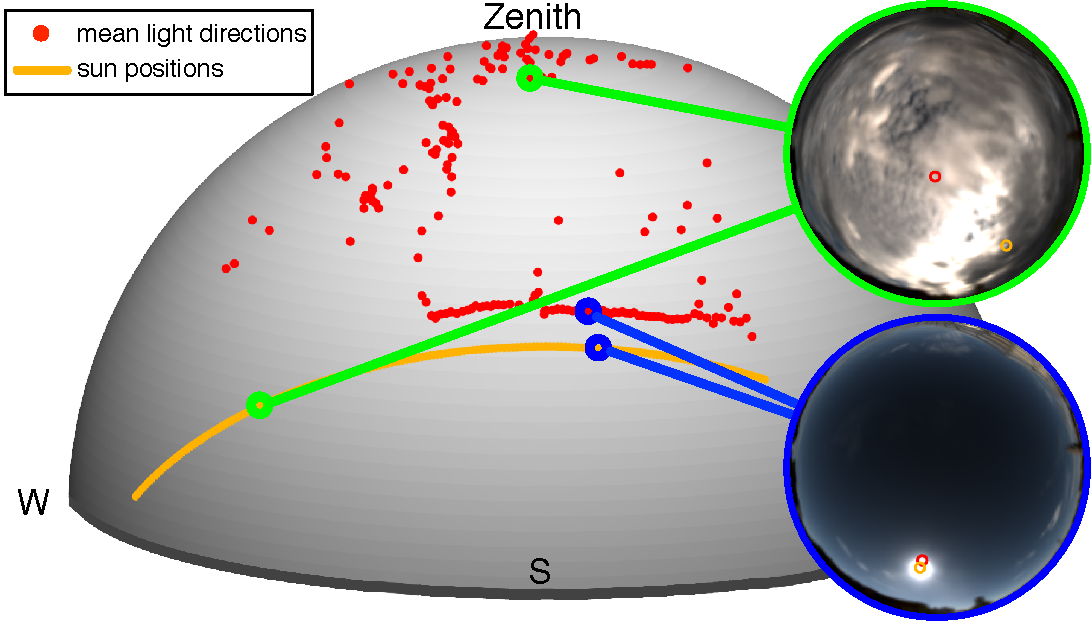
\includegraphics[width=0.5\linewidth]{./figures/mlvFig/mlvFig.pdf}
    \caption{Cloud effect on the mean light direction over one day: while the sun path (orange) yields nearly co-planar directions of illumination, the mean light directions (red dots) provide a much more varied set (data from 11/06/2013, 2nd row of fig.~\ref{fig:database}).}
    \label{fig:mlv}
\end{figure}

This key observation also demonstrates the advantages of adopting more elaborate illumination models (\eg, \cite{yu-iccp-13}). For instance, the simpler point light model was used in \cite{shen-pg-14} to study the conditioning of outdoor PS. Because the atmospheric component is not modeled, the conclusion was that single-day reconstruction breaks down in two cases of nearly coplanar sun directions: closer to the poles near the winter solstice, and worldwide near an equinox. Our results suggest that more attention should be placed on the illumination model, without focusing exclusively on the sun.

\subsubsection{Influence of sun elevation}
\label{sec:sun-elevation-results}

We also hypothesized the position of the sun to have an important effect on the ability to recover surface normals outdoors. Since our dataset is already aligned in terms of sun azimuths (see sec.~\ref{sec:hdrdb}), we now analyze the influence of sun elevation. For this purpose, we retain only the days for which the sun visibility was between 15--85\% of the time. We then compute the relation between sun elevation and expected reconstruction confidence, as illustrated in fig.~\ref{fig:sun-elevation-plot}.

Sun elevation does appear to have an influence, with higher sun elevations resulting in slightly increased uncertainty than when the sun is lower in the sky. However, the impact is less drastic than that of cloud cover from sec.~\ref{sec:cloud-cover-results}. These results can be explained, at least in part, by the smaller sun-zenith shift introduced by cloud cover when the sun is already high in the sky; therefore, smaller improvements in conditioning are obtained.

Our data-driven analysis shows that higher sun elevations---predicted as preferable by the analysis in~\cite{shen-pg-14}---are in fact not necessarily optimal when taking more elaborate illumination models into account.


% Section 3 has a note about non-coplanar sun directions  vs  non-coplanar mean light vectors (zenith, sun elevation),


\subsubsection{Analyzing full objects}

So far, our analysis has focused solely on one patch (one normal direction) at a time. But can we also say something about an entire object? Clearly, a full answer to this question would require analyzing non-local effects such as occlusions, inter-reflections, cast shadows, etc. However, we hypothesize that a simpler analysis ignoring these effects can still provide useful results. We therefore predict the performance of an outdoor PS algorithm by computing the expected value of the confidence interval, $\mathbb{E}_{\bf n}[\mathcal{C}_{\bf n}]$, over an entire object; expectation over the normal vector is computed using a prior distribution taken from a simpler convex shape (\eg, a sphere). Fig.~\ref{fig:objects} shows the expected reconstruction performance for two objects: a bottle, and the bunny. Overall, surface reconstruction performance is expected to be best when objects face south (\ie, the sun).

\begin{figure}[t]
    \centering
    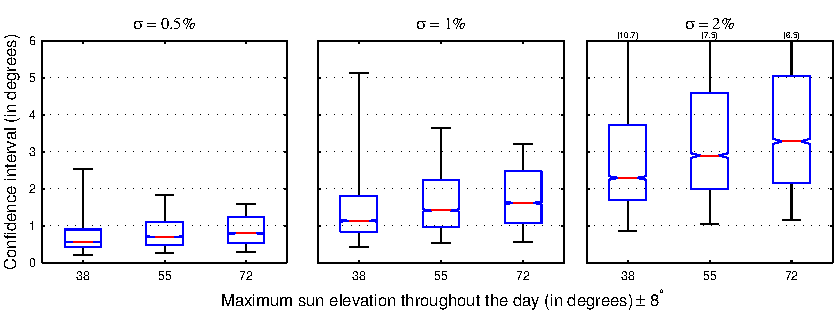
\includegraphics[width=\linewidth]{./figures/confidenceIntervals/sunElevationPlot-topHemisphere.pdf}
    \caption{Median confidence interval of normal estimates (red line) as a function of maximum sun elevation over the course of the day for various values of $\sigma$. Although the effect is not as significant as with cloud cover, we anticipate a small decrease in performance at higher sun elevations. The lower (upper) edge of each blue box indicates the 25th (75th) percentile. Statistics are computed only on normals pointing upwards to lessen ground effects.}
    \label{fig:sun-elevation-plot}
\end{figure}

% \begin{figure}[t]
%     \centering
%     \begin{sideways}\begin{minipage}{.45\linewidth}\centering \scriptsize Low elevation \vspace{5pt} \end{minipage}\end{sideways}
%     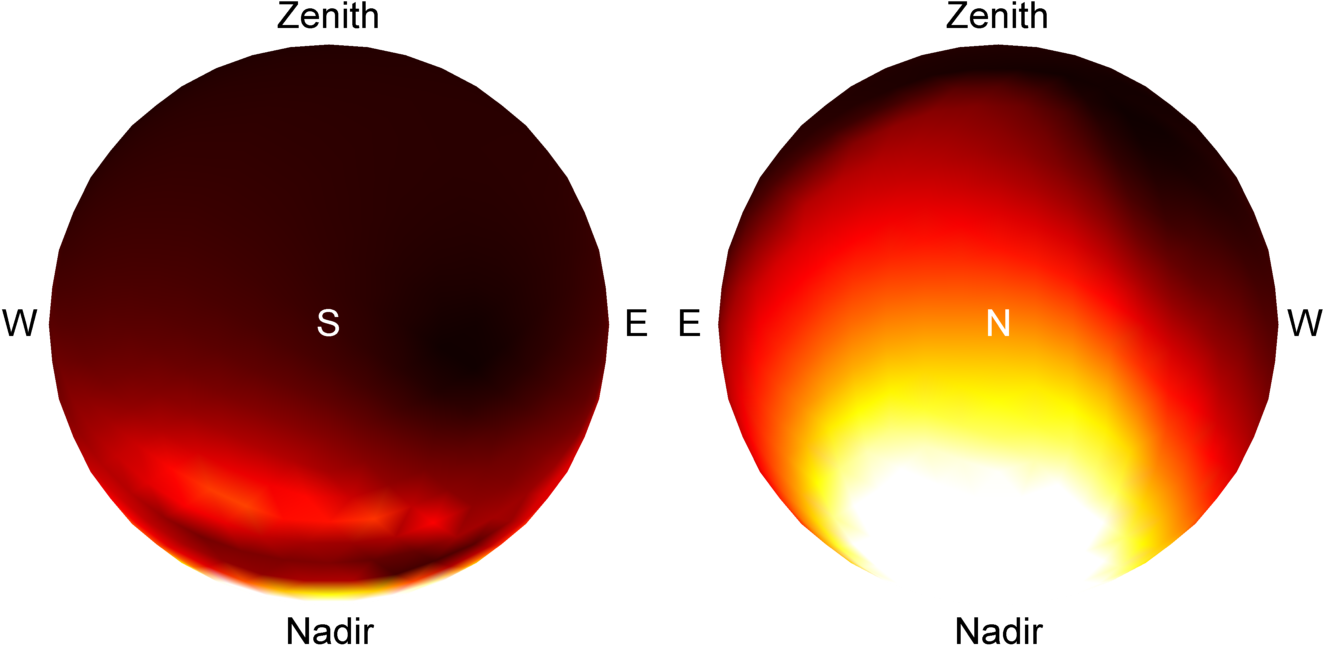
\includegraphics[width=.9\linewidth]{./figures/confidenceIntervals/elevation-low-mean_10pm.png} \\[2mm]
%     \begin{sideways}\begin{minipage}{.45\linewidth}\centering \scriptsize High elevation \vspace{5pt} \end{minipage}\end{sideways}
%     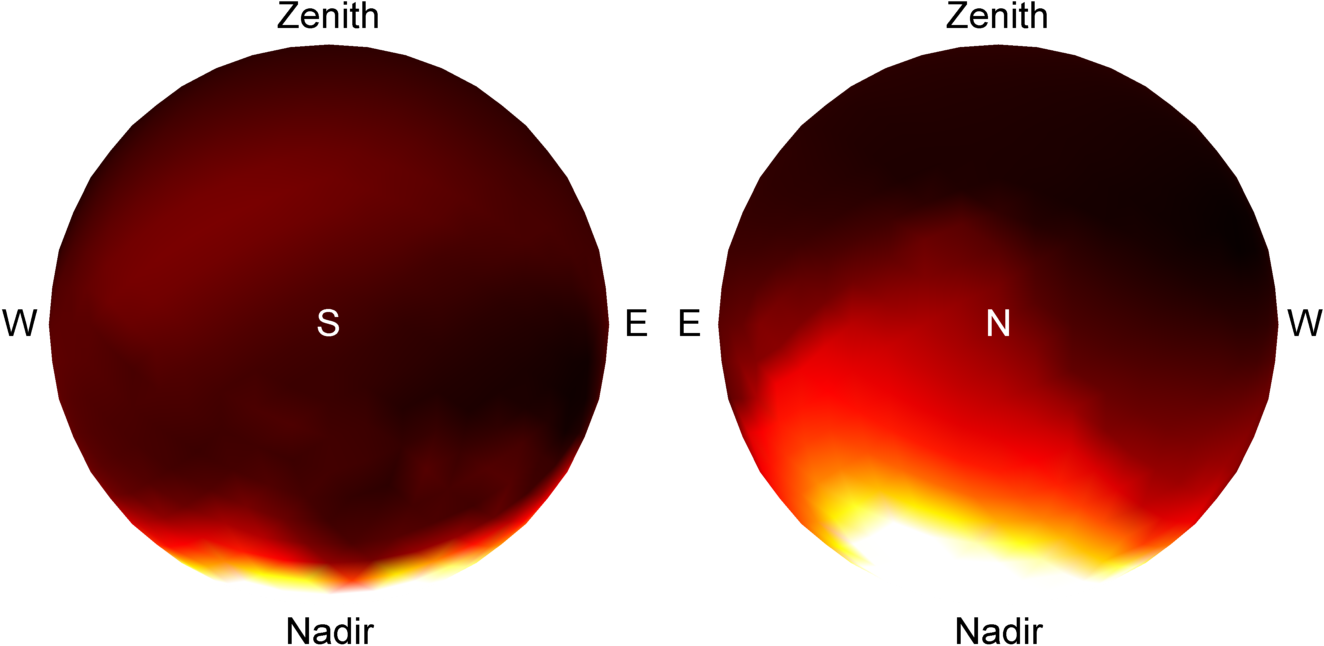
\includegraphics[width=.9\linewidth]{./figures/confidenceIntervals/elevation-high-mean_10pm.png} \\[3mm]
%     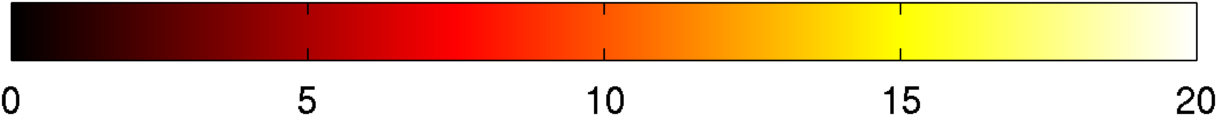
\includegraphics[width=\linewidth]{./figures/confidenceIntervals/colorbar.png}
%   \caption{Influence of sun elevation on the 95\% confidence intervals with $\sigma=1\%$. The top plot shows the mean, per-normal, confidence intervals obtained for mixed skies with low sun elevation. The bottom plot shows the same data, but for mixed skies with high sun elevation. As in fig.~\ref{fig:confidence-intervals}, the plots show the full sphere of normals from two different viewpoints: South (left), and North (right). Cardinal directions are shown for reference. The color-coding is indicated below the plots.}
%   \label{fig:sun-elevation}
% \end{figure}

\begin{figure}[t]
    \centering
    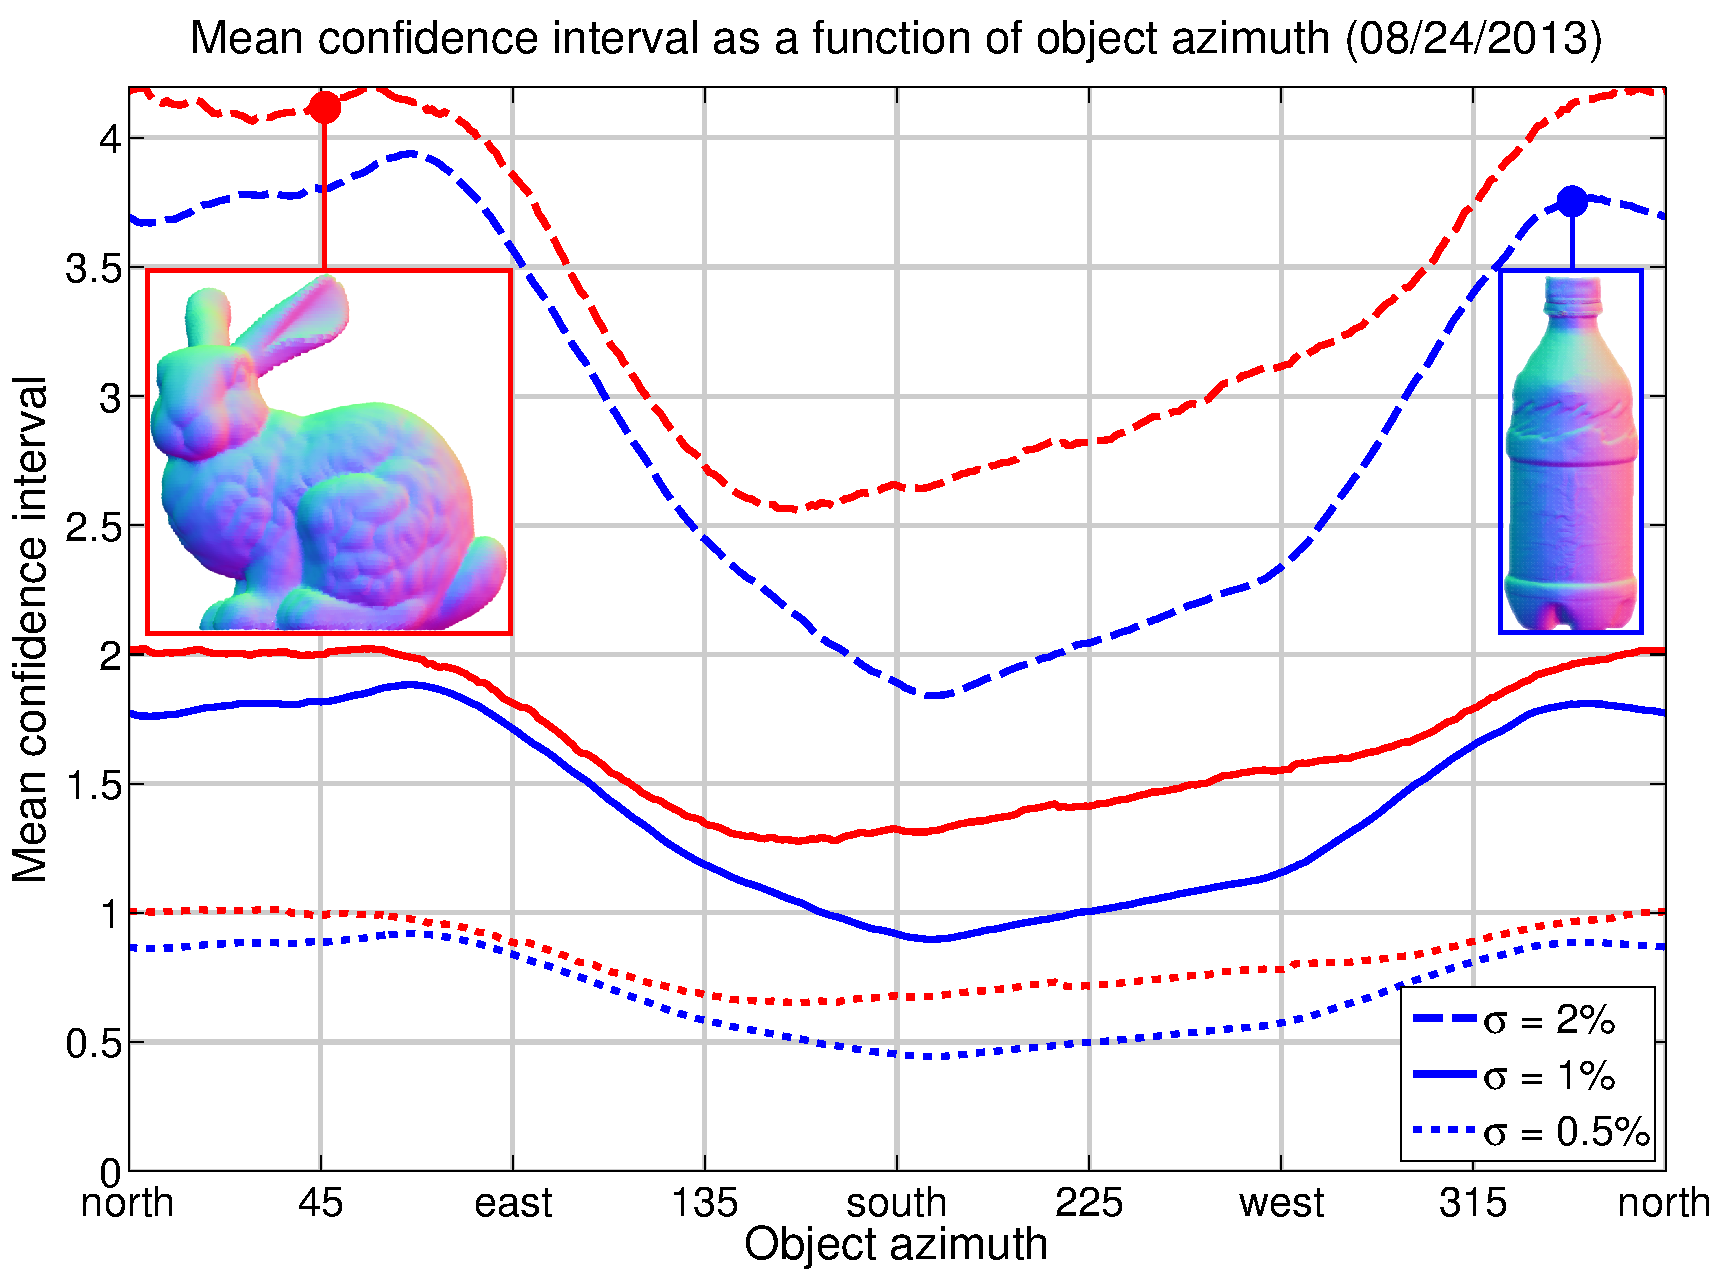
\includegraphics[width=\linewidth]{./figures/objectFig/objectFigNoise.pdf}
    \caption{Predicting object reconstruction performance for the 08/24/2013 dataset. These curves show the mean surface reconstruction variance for two objects: a bottle (blue) and the bunny (red). Irrespective of the noise level, surface reconstruction performance is expected to be best when the objects face south.}
    \label{fig:objects}
\end{figure}

\subsection{Validation on real object images}
\label{sec:validation}

The analysis performed on our dataset indicates that surface patches may be better reconstructed in certain conditions, dependent upon cloud coverage, sun elevation, and the orientation of the patch itself. At the time of this writing, a thorough validation on real outdoor images of different objects is currently under development. This section reports preliminary results on real outdoor images of an owl statuette (fig.~\ref{fig:reconstruction:example_envmaps}), which was scanned with a Creaform MetraSCAN at a resolution of 0.05mm to provide a reference of true surface orientation.

\begin{figure*}[!ht]
    \centering
    \setlength{\tabcolsep}{0pt}
    \newcommand{\customwidth}{.08\linewidth}
    \begin{tabular}{@{}rcccccccccccc@{}}
    &
    \begin{minipage}{\customwidth}\centering\scriptsize 10:30 \end{minipage} &
    \begin{minipage}{\customwidth}\centering\scriptsize 11:00 \end{minipage} &
    \begin{minipage}{\customwidth}\centering\scriptsize 11:30 \end{minipage} &
    \begin{minipage}{\customwidth}\centering\scriptsize 12:00 \end{minipage} &
    \begin{minipage}{\customwidth}\centering\scriptsize 12:30 \end{minipage} &
    \begin{minipage}{\customwidth}\centering\scriptsize 13:00 \end{minipage} &
    \begin{minipage}{\customwidth}\centering\scriptsize 13:30 \end{minipage} &
    \begin{minipage}{\customwidth}\centering\scriptsize 14:00 \end{minipage} &
    \begin{minipage}{\customwidth}\centering\scriptsize 14:30 \end{minipage} &
    \begin{minipage}{\customwidth}\centering\scriptsize 15:00 \end{minipage} &
    \begin{minipage}{\customwidth}\centering\scriptsize 15:30 \end{minipage} &
    \begin{minipage}{\customwidth}\centering\scriptsize 16:00 \end{minipage}
    \\
    \begin{sideways}\begin{minipage}{\customwidth}\centering \scriptsize illumination \\ 43\% sun vis. \\ \vspace{5pt} \end{minipage}\end{sideways} &
    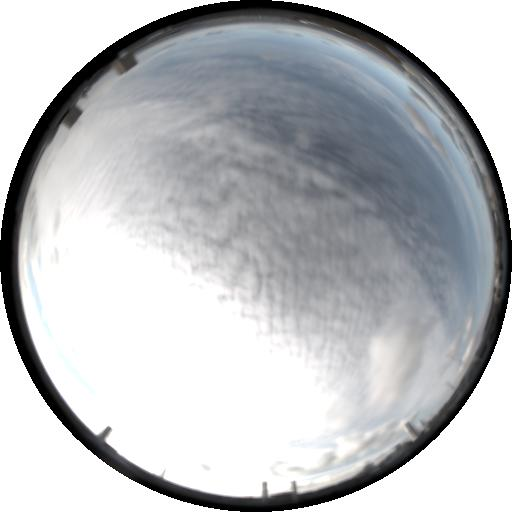
\includegraphics[width=\customwidth]{./figures/reconstruction/envmaps/20141011_102928.jpg} &
    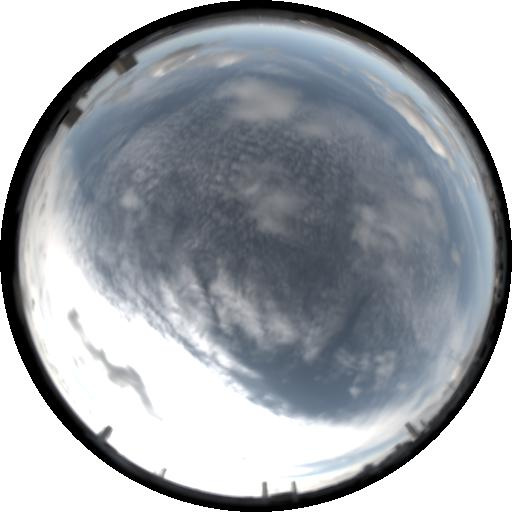
\includegraphics[width=\customwidth]{./figures/reconstruction/envmaps/20141011_110128.jpg} &
    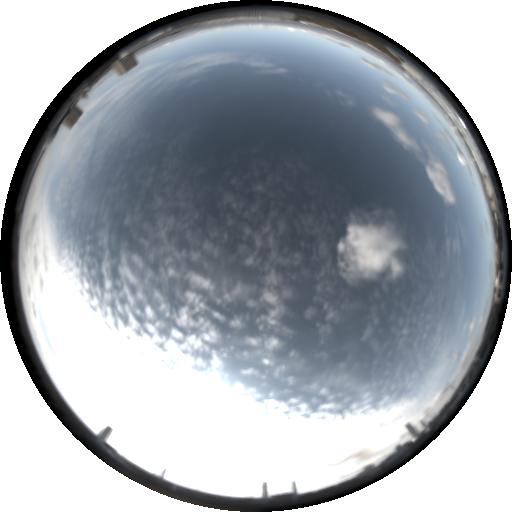
\includegraphics[width=\customwidth]{./figures/reconstruction/envmaps/20141011_112928.jpg} &
    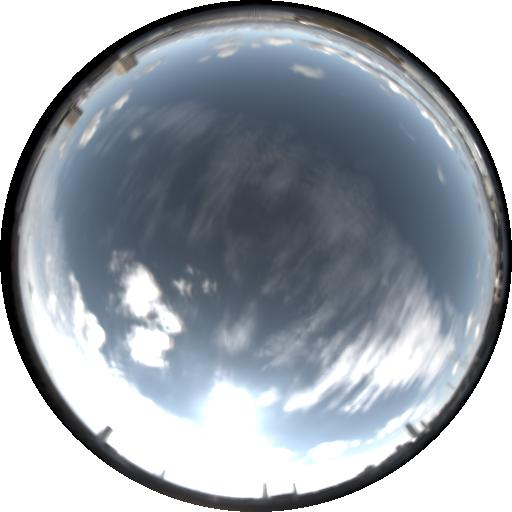
\includegraphics[width=\customwidth]{./figures/reconstruction/envmaps/20141011_120128.jpg} &
    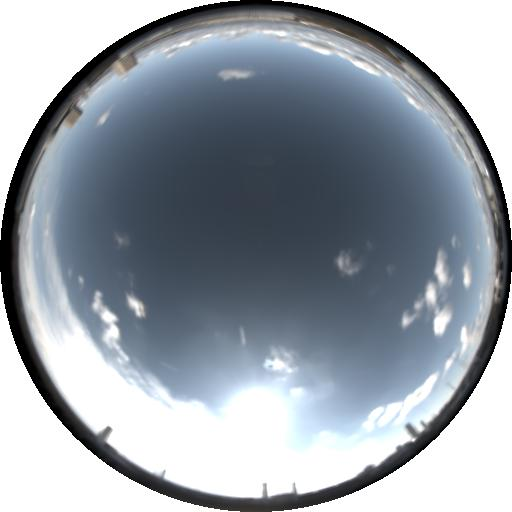
\includegraphics[width=\customwidth]{./figures/reconstruction/envmaps/20141011_122929.jpg} &
    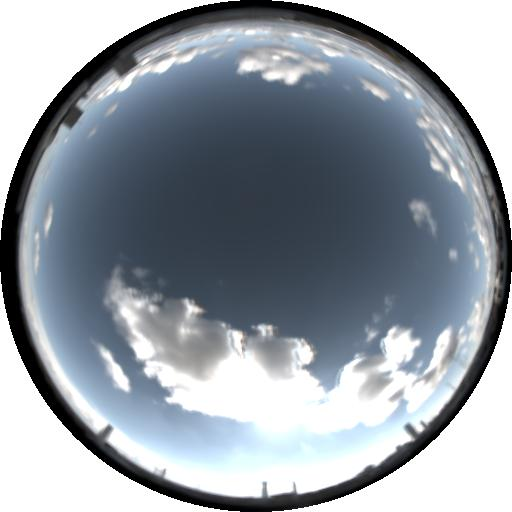
\includegraphics[width=\customwidth]{./figures/reconstruction/envmaps/20141011_130128.jpg} &
    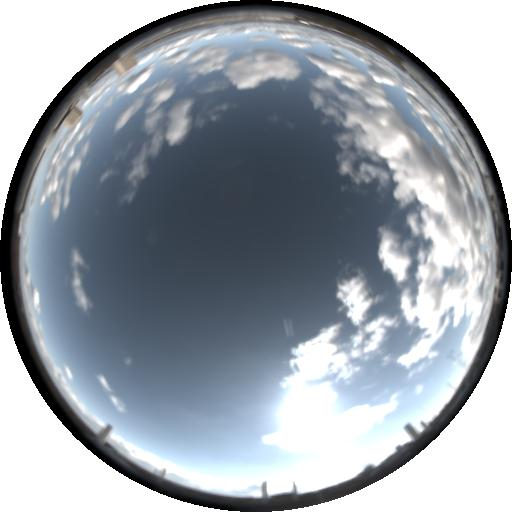
\includegraphics[width=\customwidth]{./figures/reconstruction/envmaps/20141011_132928.jpg} &
    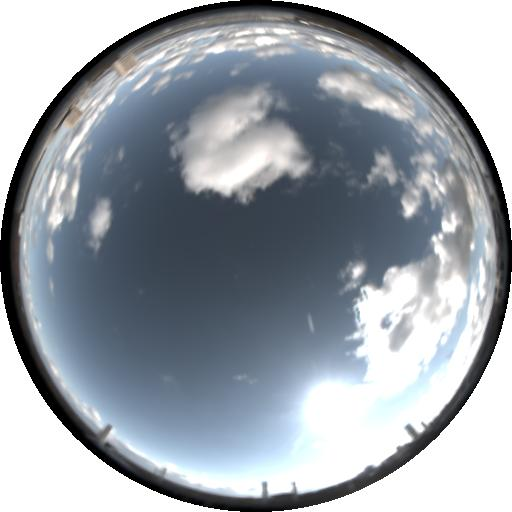
\includegraphics[width=\customwidth]{./figures/reconstruction/envmaps/20141011_135928.jpg} &
    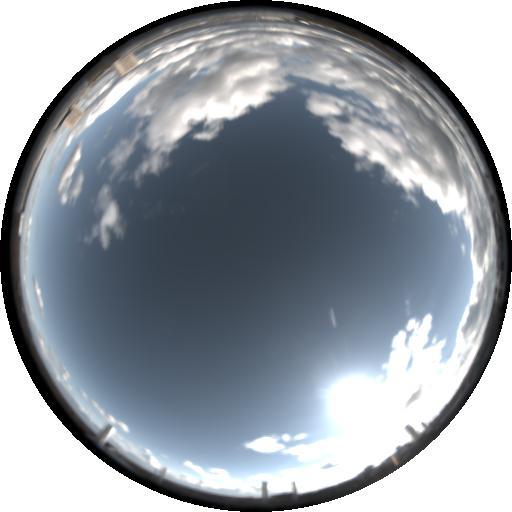
\includegraphics[width=\customwidth]{./figures/reconstruction/envmaps/20141011_142928.jpg} &
    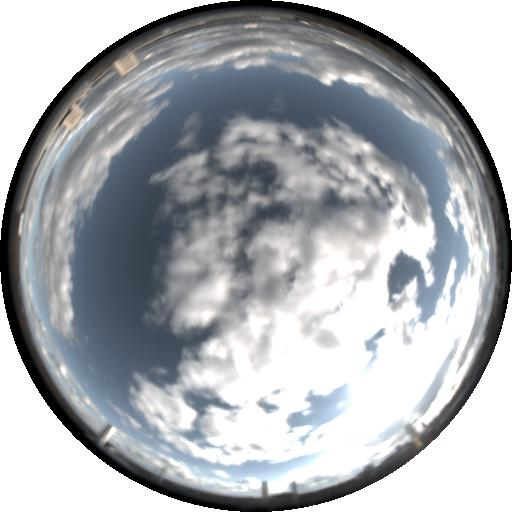
\includegraphics[width=\customwidth]{./figures/reconstruction/envmaps/20141011_145928.jpg} &
    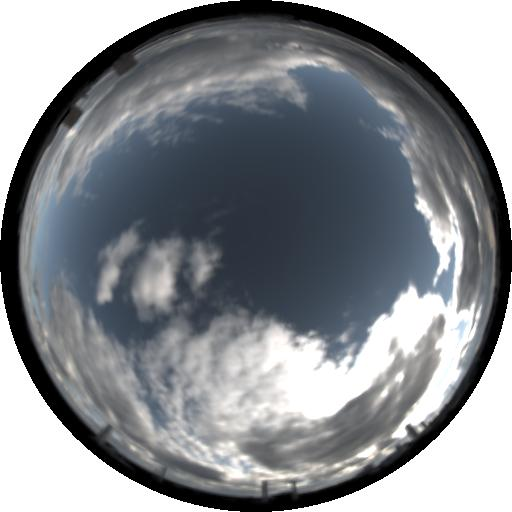
\includegraphics[width=\customwidth]{./figures/reconstruction/envmaps/20141011_152928.jpg} &
    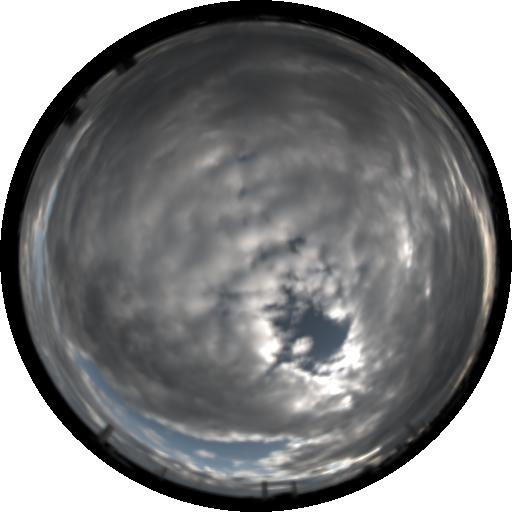
\includegraphics[width=\customwidth]{./figures/reconstruction/envmaps/20141011_155928.jpg}
    \\
    \begin{sideways}\begin{minipage}{.106\linewidth}\centering \scriptsize object capture \\ \vspace{1em} \vspace{5pt} \end{minipage}\end{sideways} &
    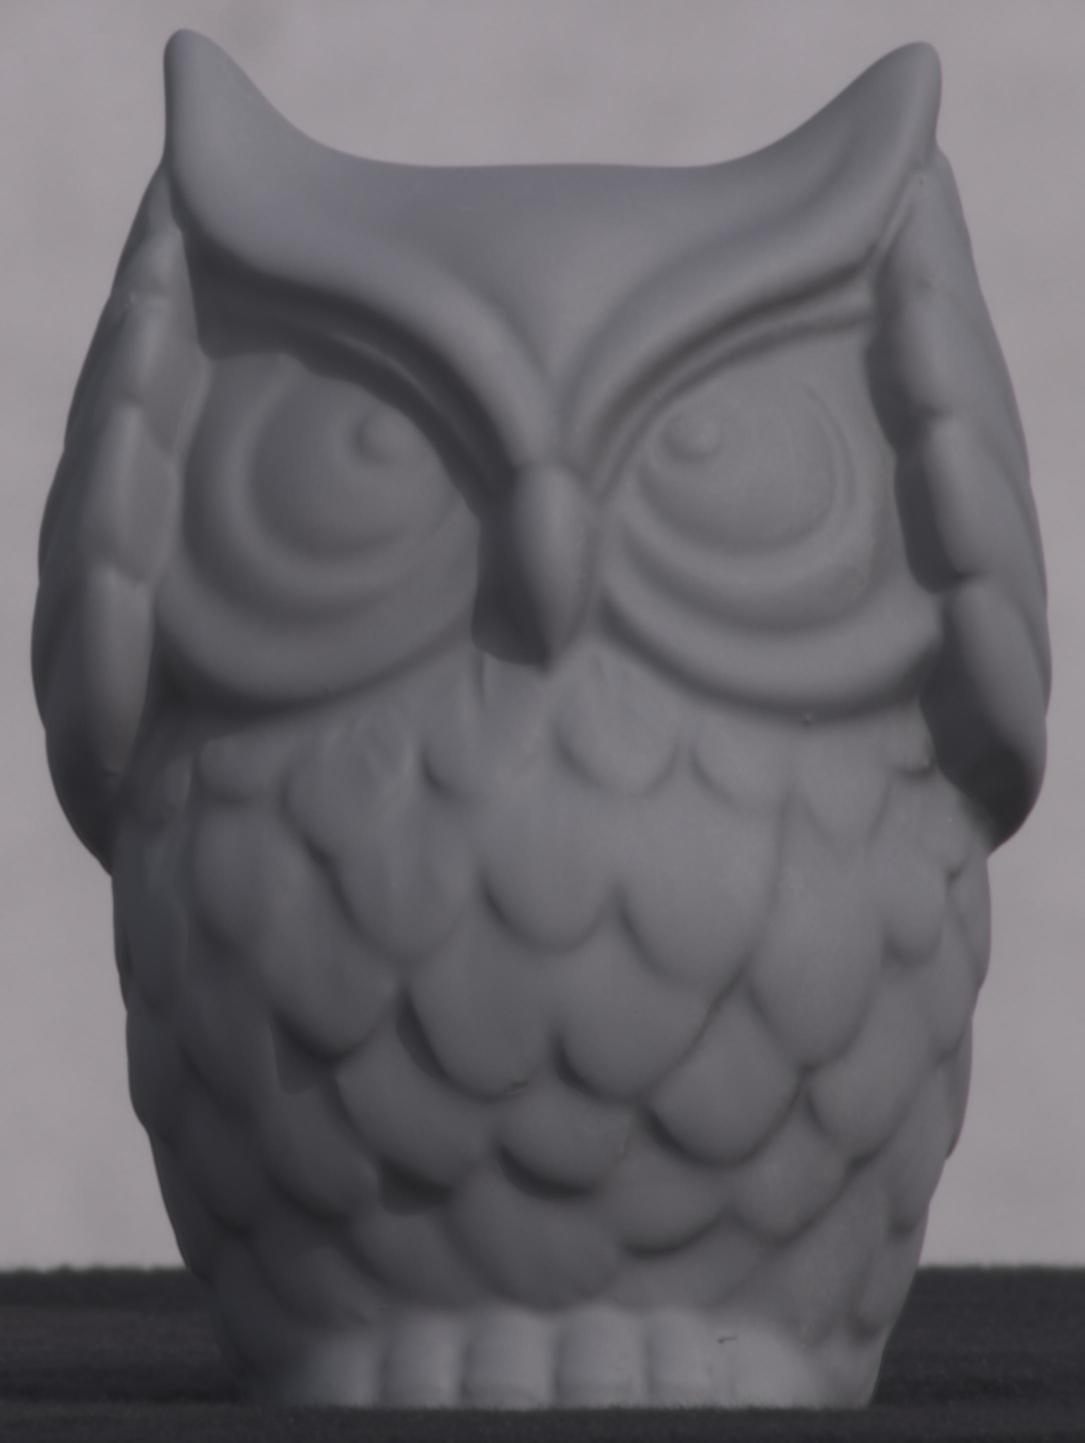
\includegraphics[width=\customwidth]{./figures/reconstruction/object/103307.jpg} &
    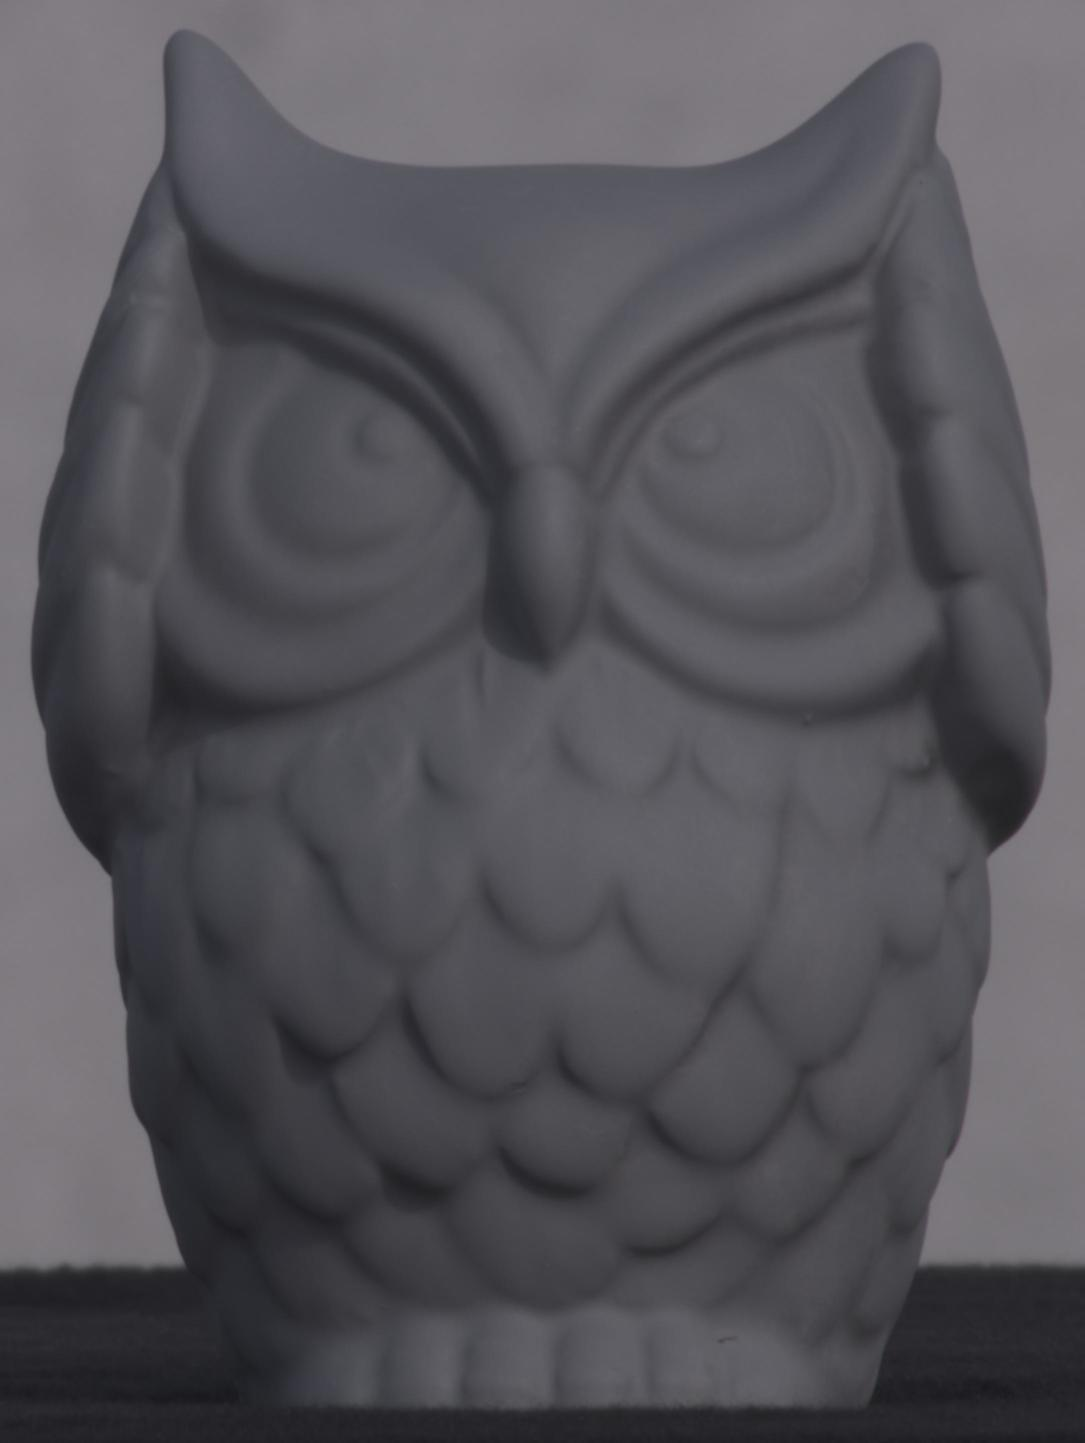
\includegraphics[width=\customwidth]{./figures/reconstruction/object/110346.jpg} &
    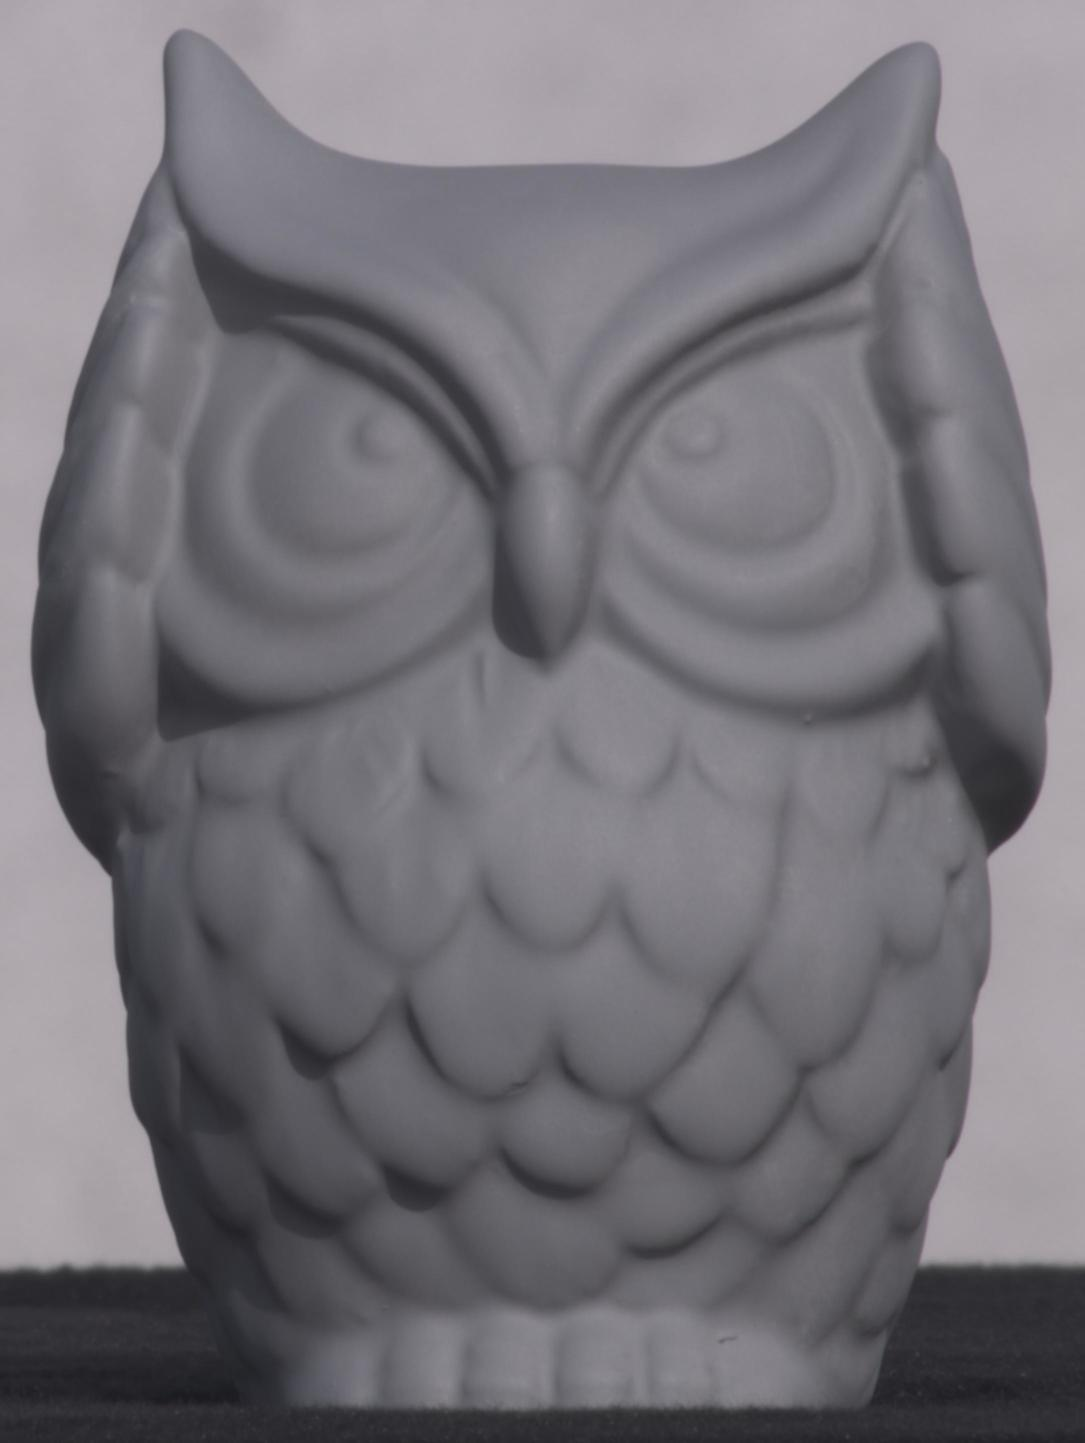
\includegraphics[width=\customwidth]{./figures/reconstruction/object/113346.jpg} &
    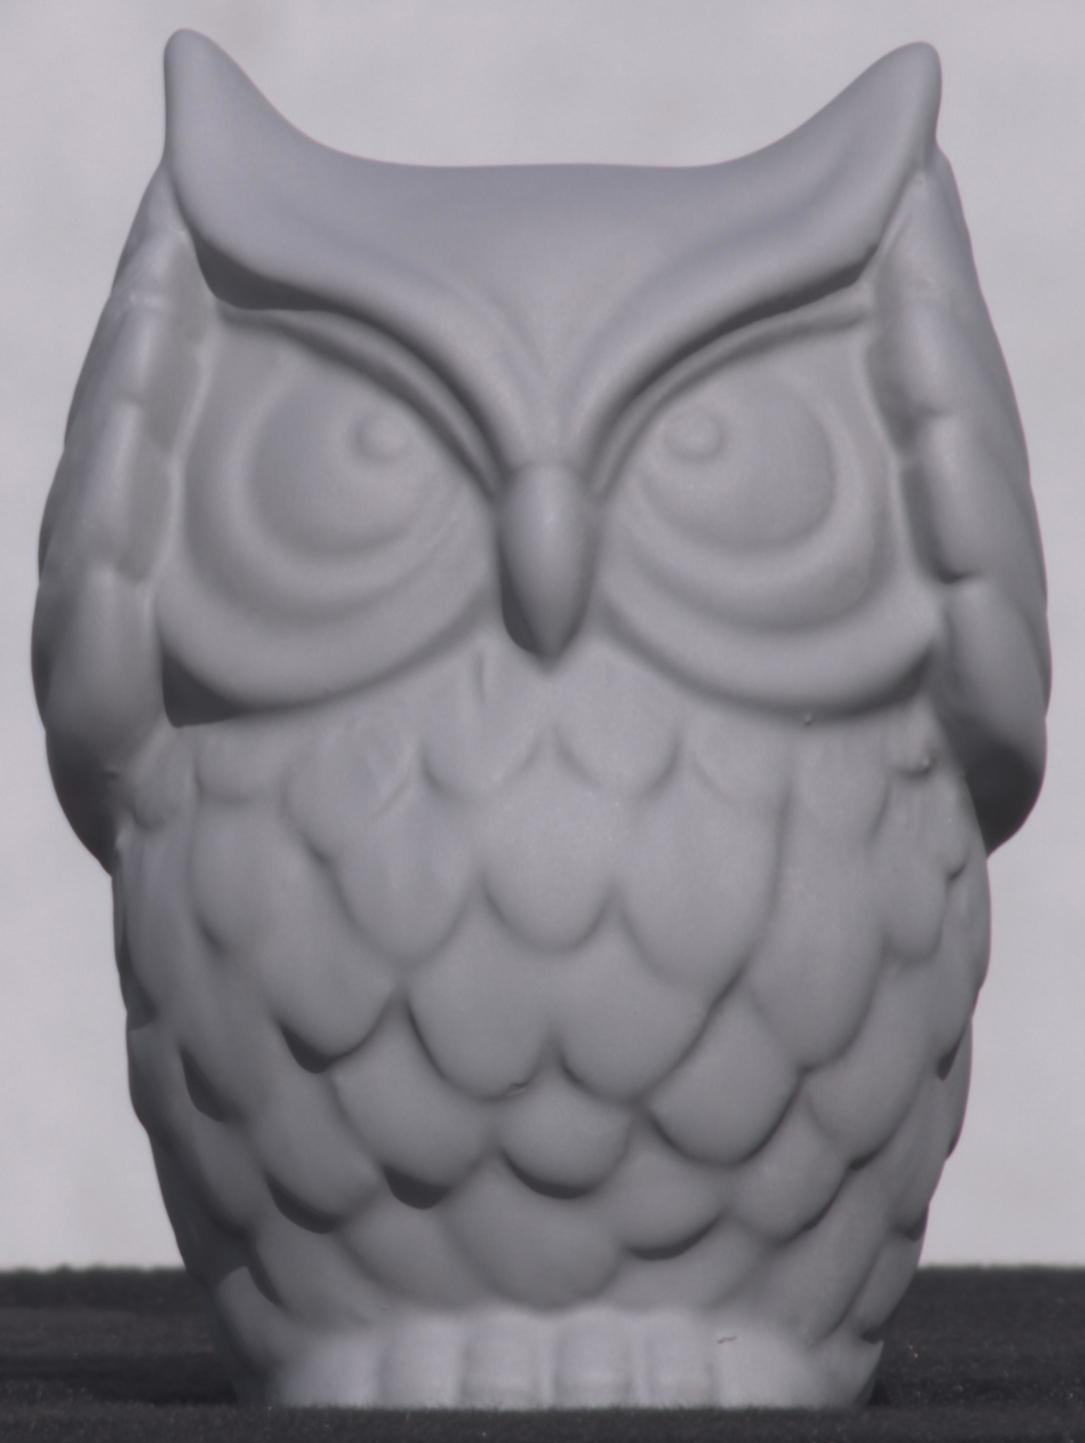
\includegraphics[width=\customwidth]{./figures/reconstruction/object/120346.jpg} &
    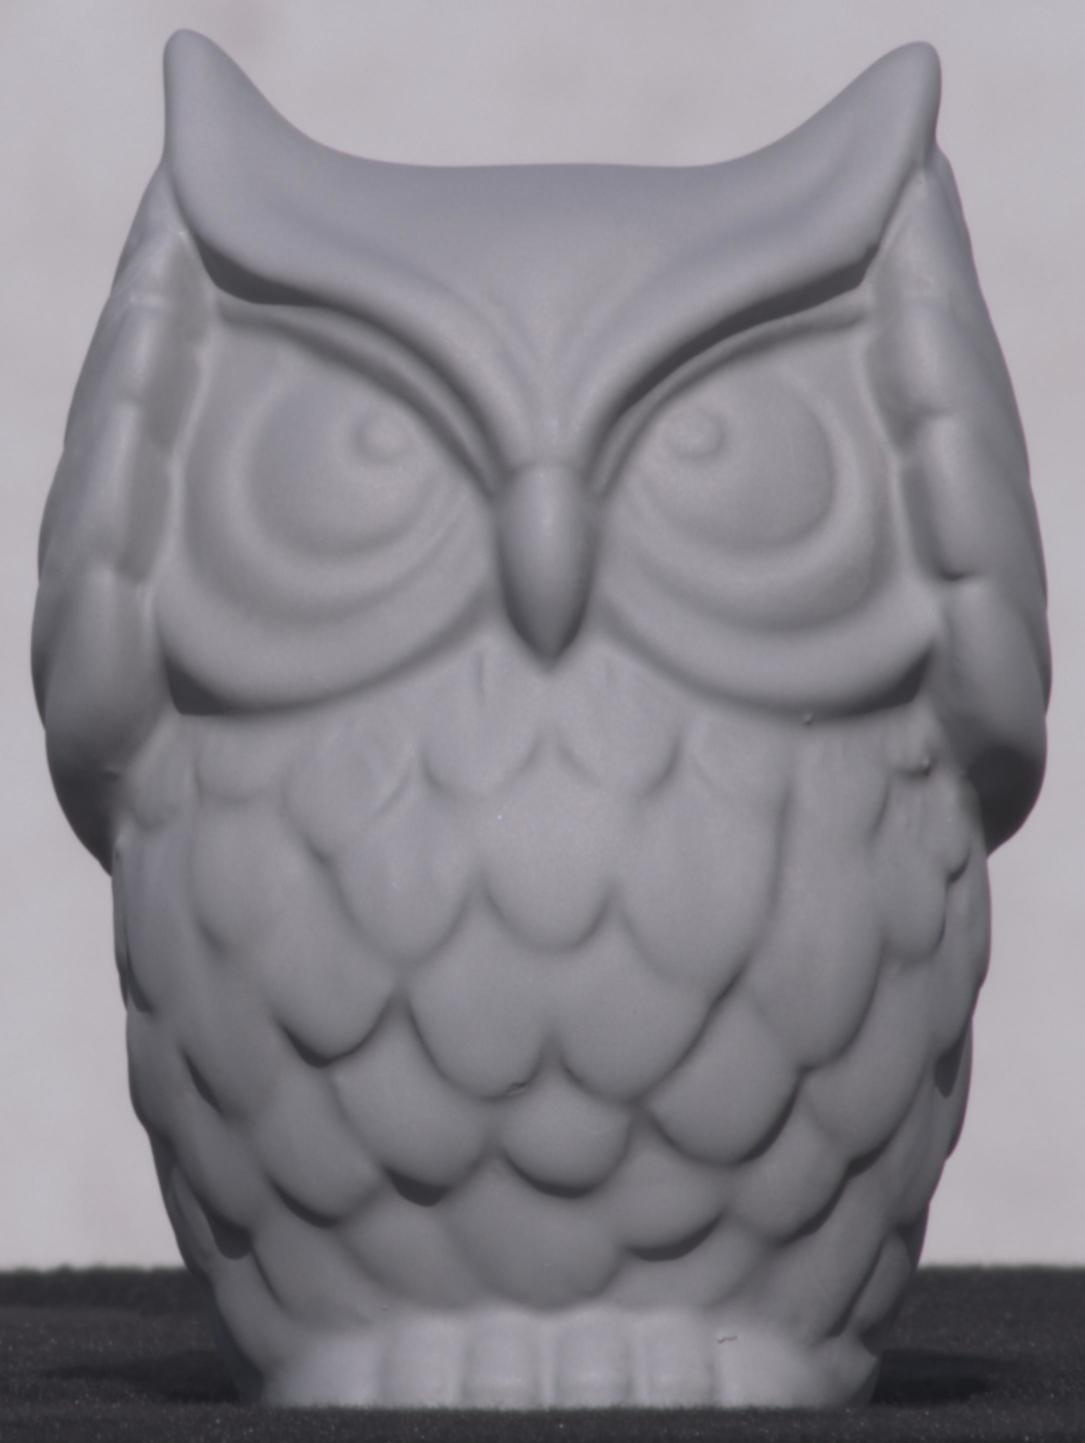
\includegraphics[width=\customwidth]{./figures/reconstruction/object/123346.jpg} &
    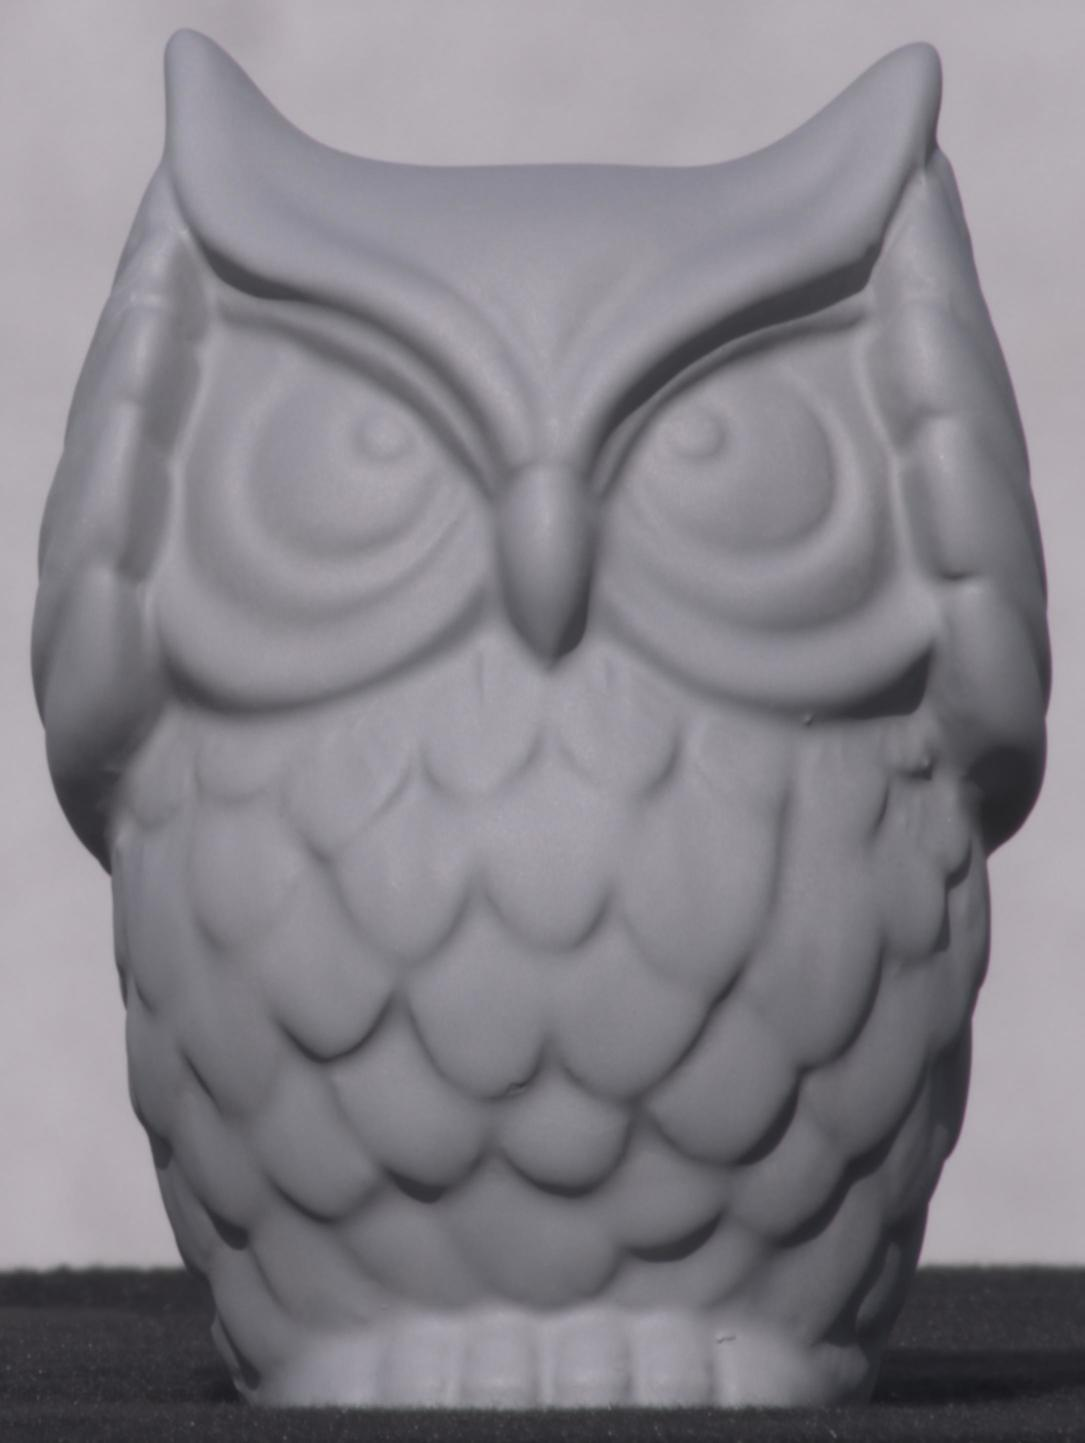
\includegraphics[width=\customwidth]{./figures/reconstruction/object/130215.jpg} &
    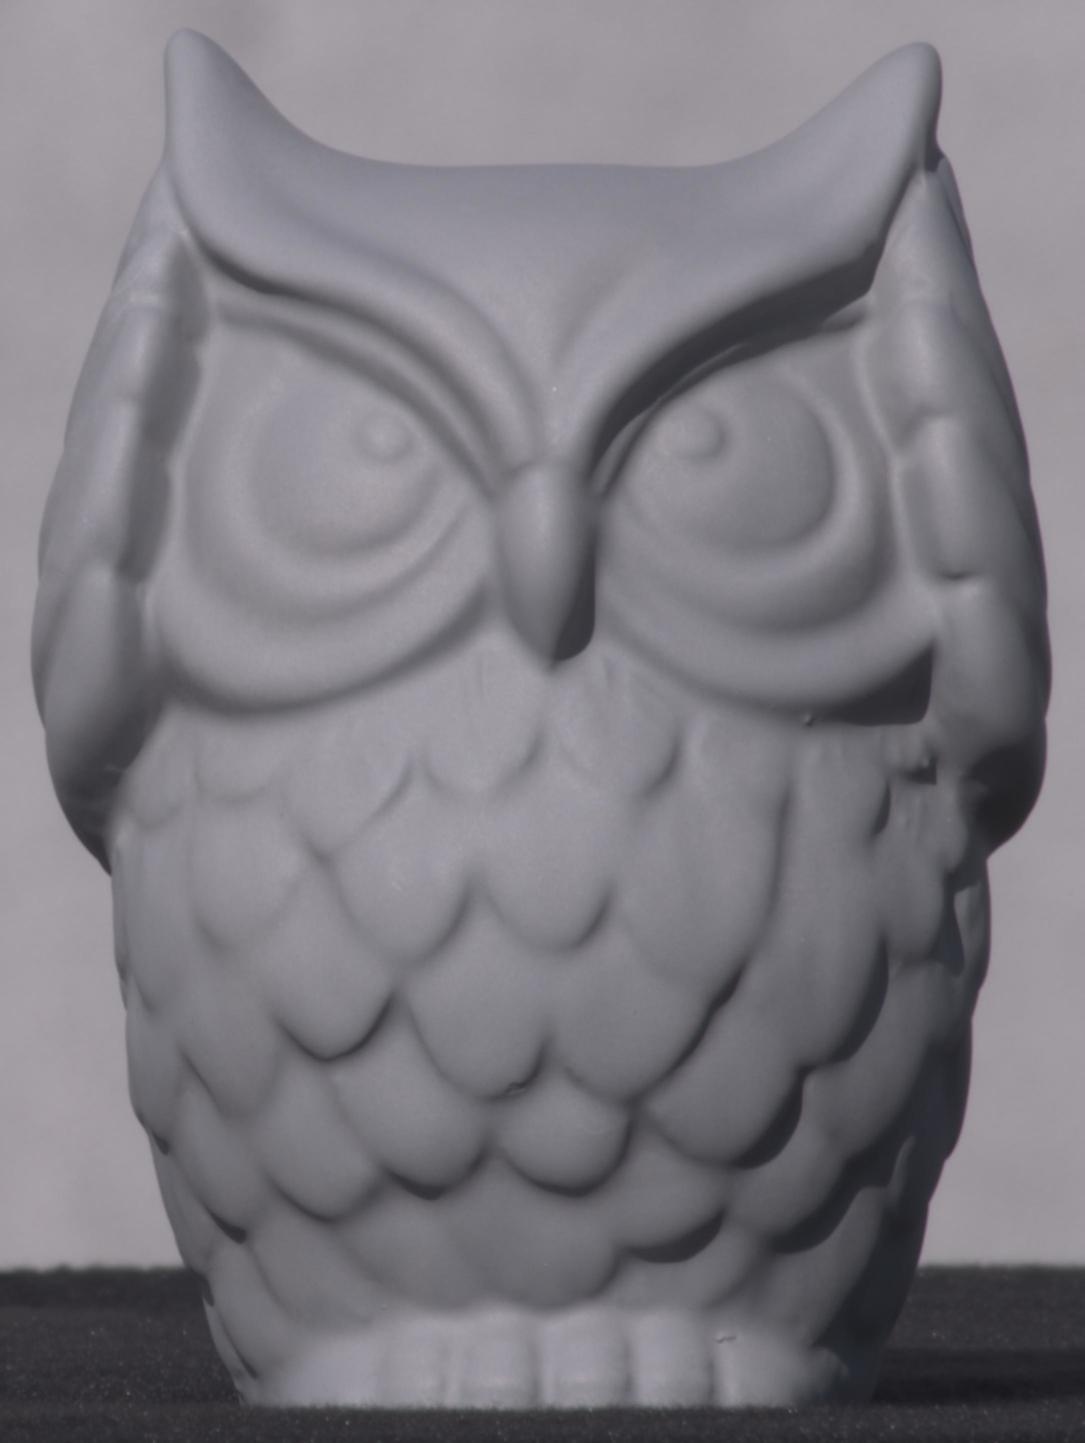
\includegraphics[width=\customwidth]{./figures/reconstruction/object/133215.jpg} &
    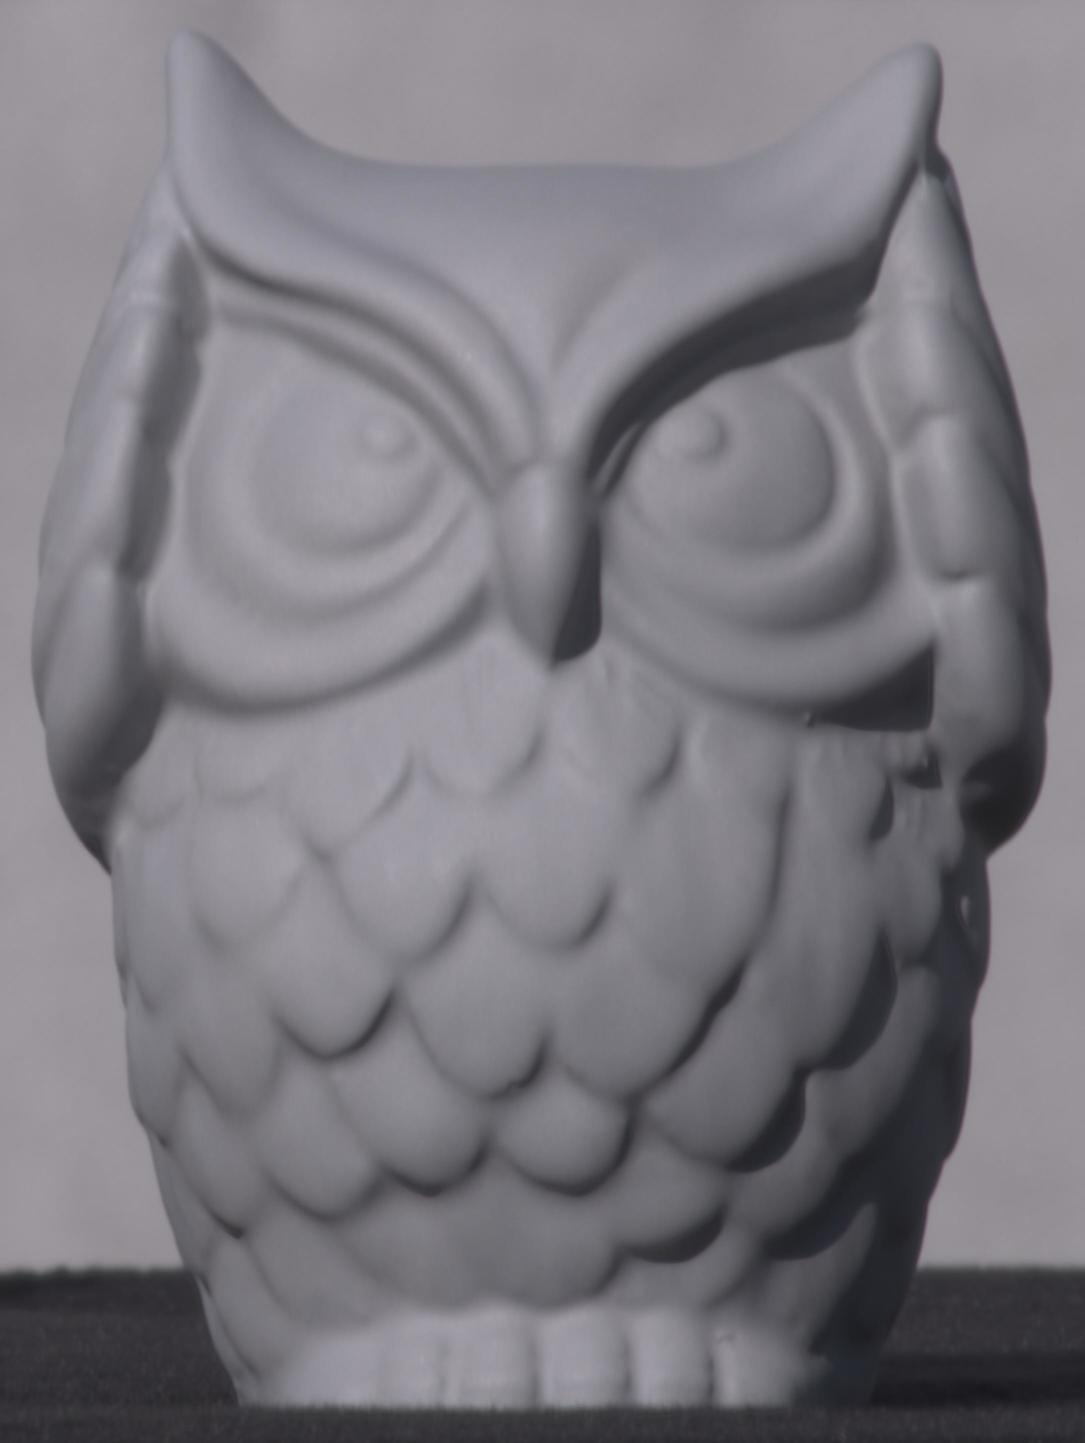
\includegraphics[width=\customwidth]{./figures/reconstruction/object/135615.jpg} &
    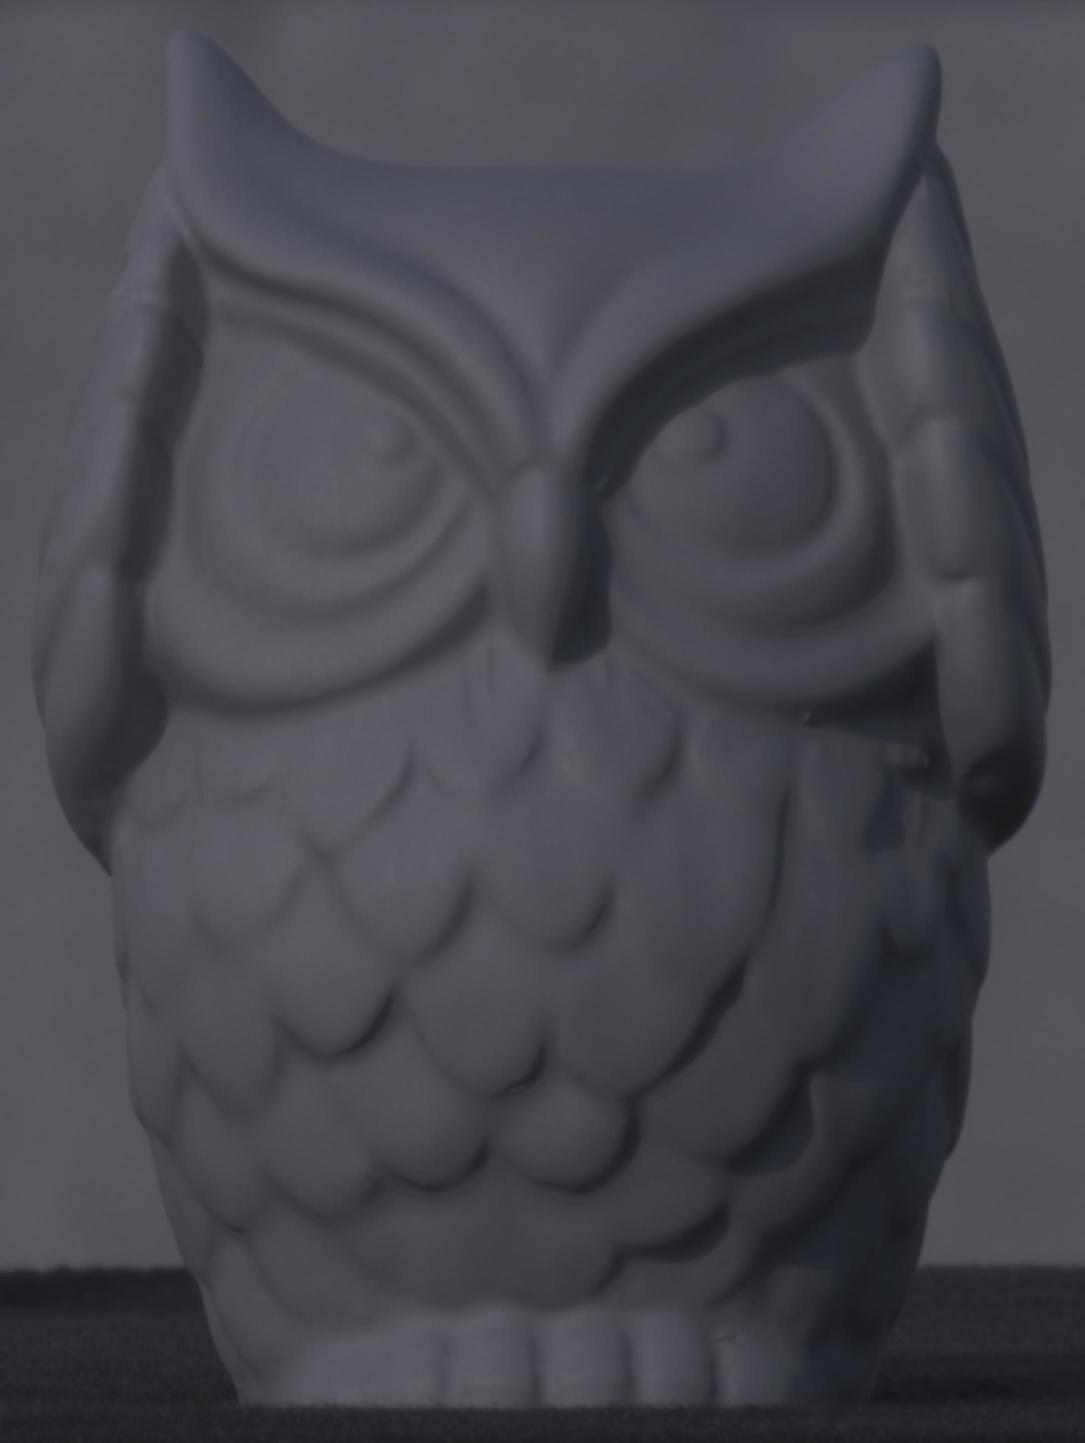
\includegraphics[width=\customwidth]{./figures/reconstruction/object/143215.jpg} &
    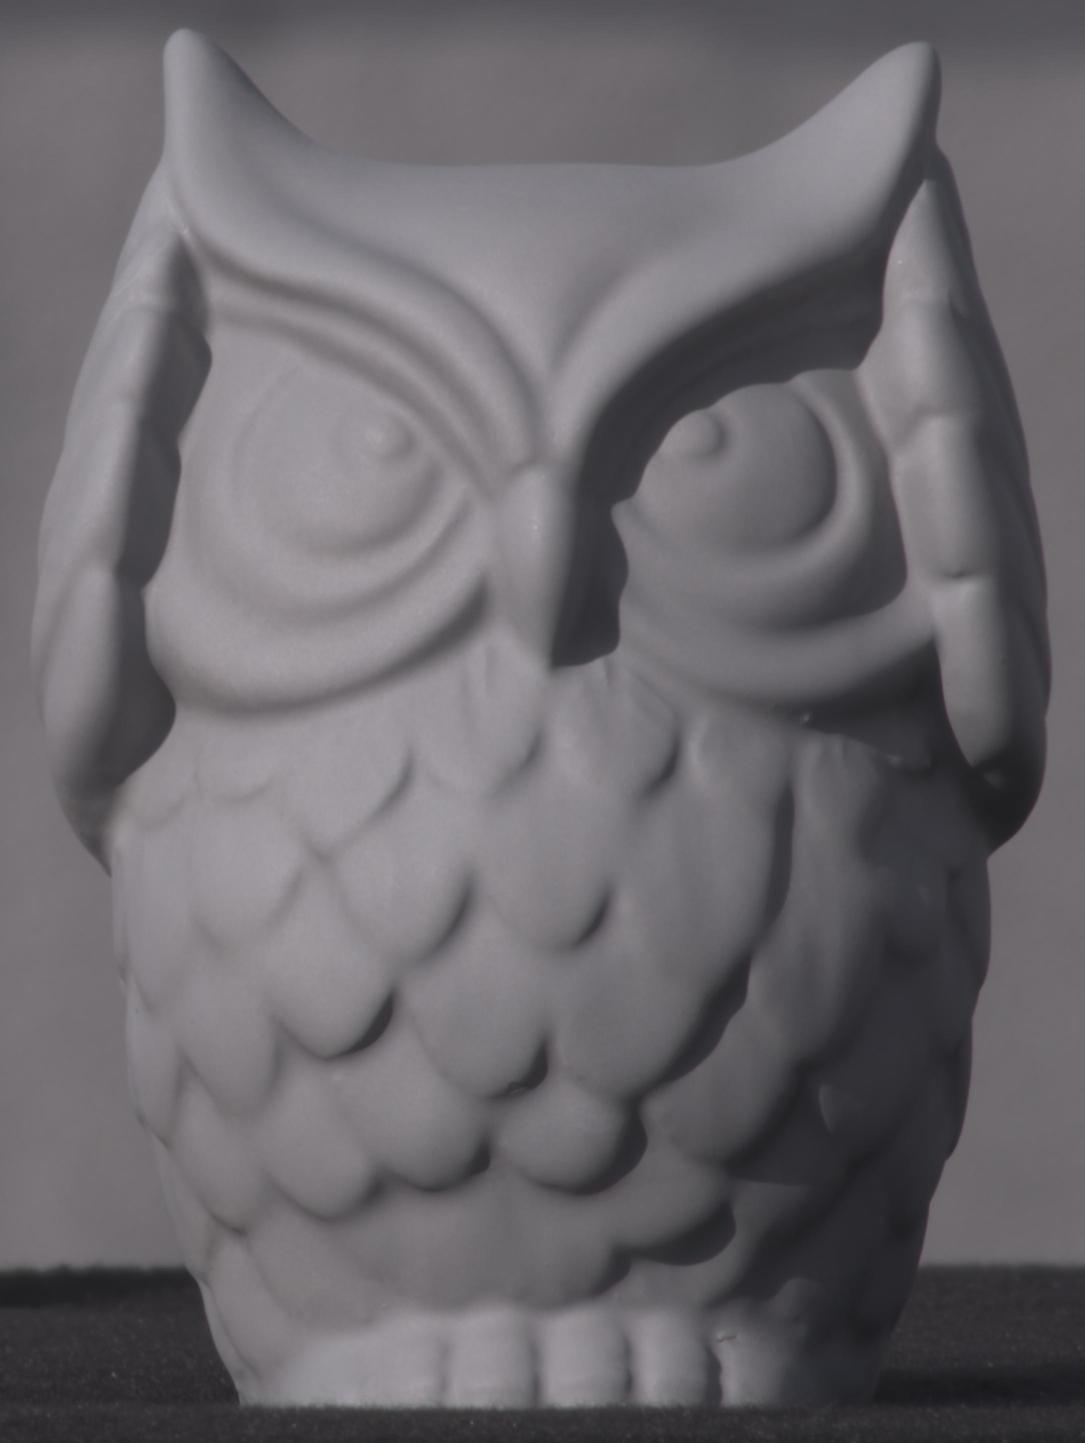
\includegraphics[width=\customwidth]{./figures/reconstruction/object/150215.jpg} &
    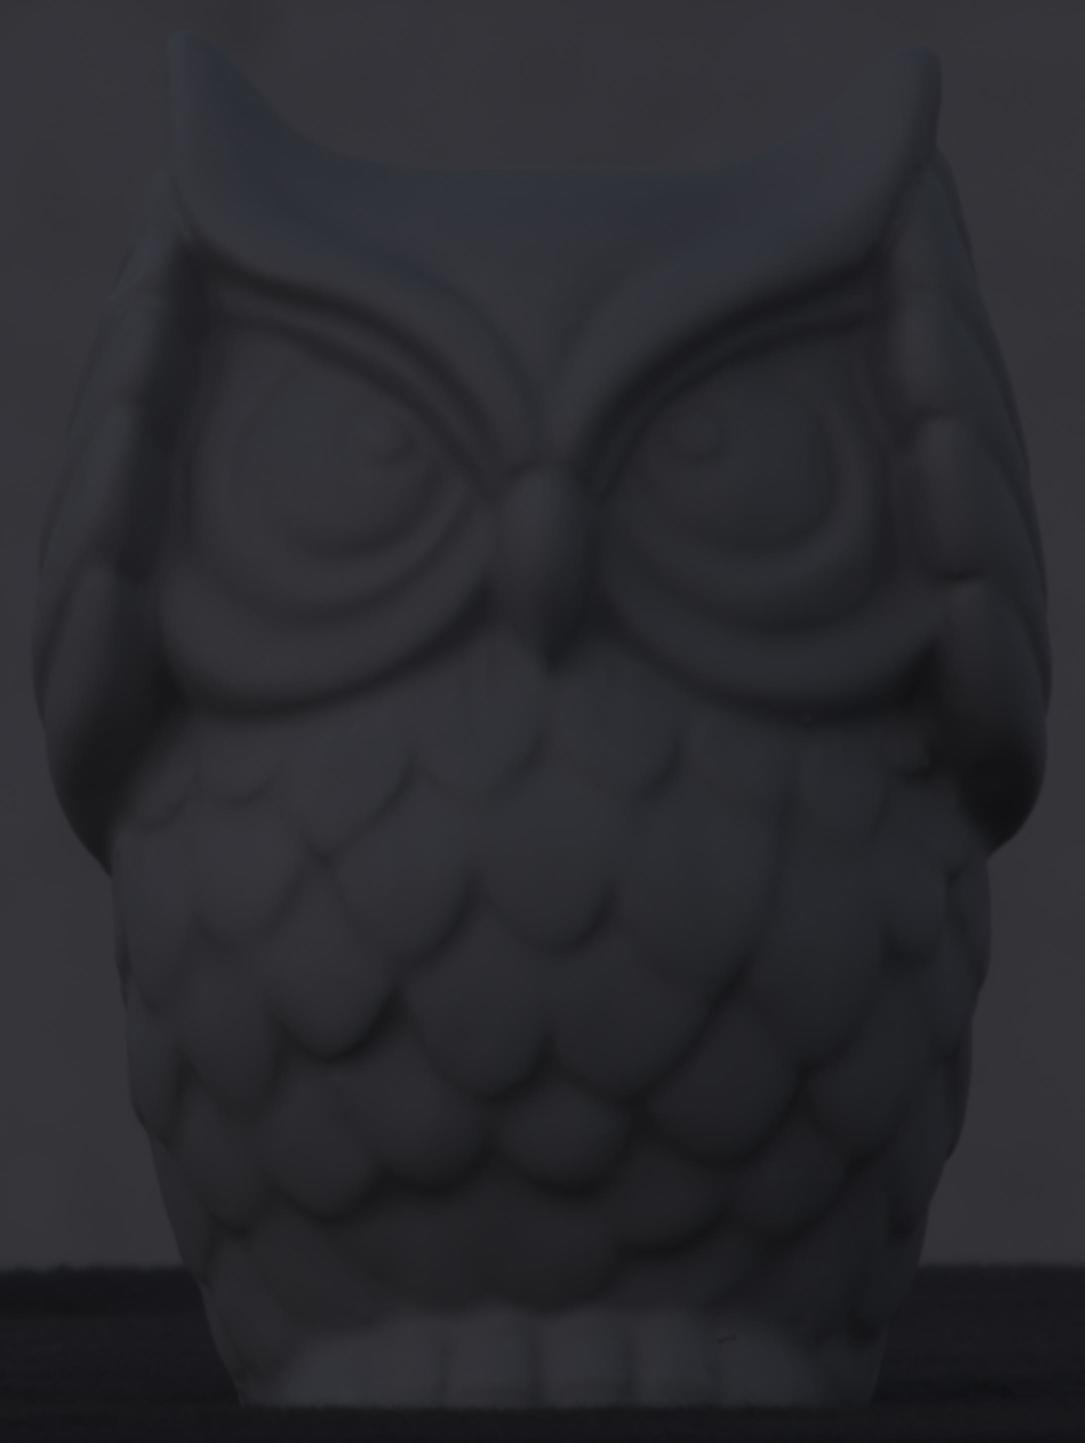
\includegraphics[width=\customwidth]{./figures/reconstruction/object/153215.jpg} &
    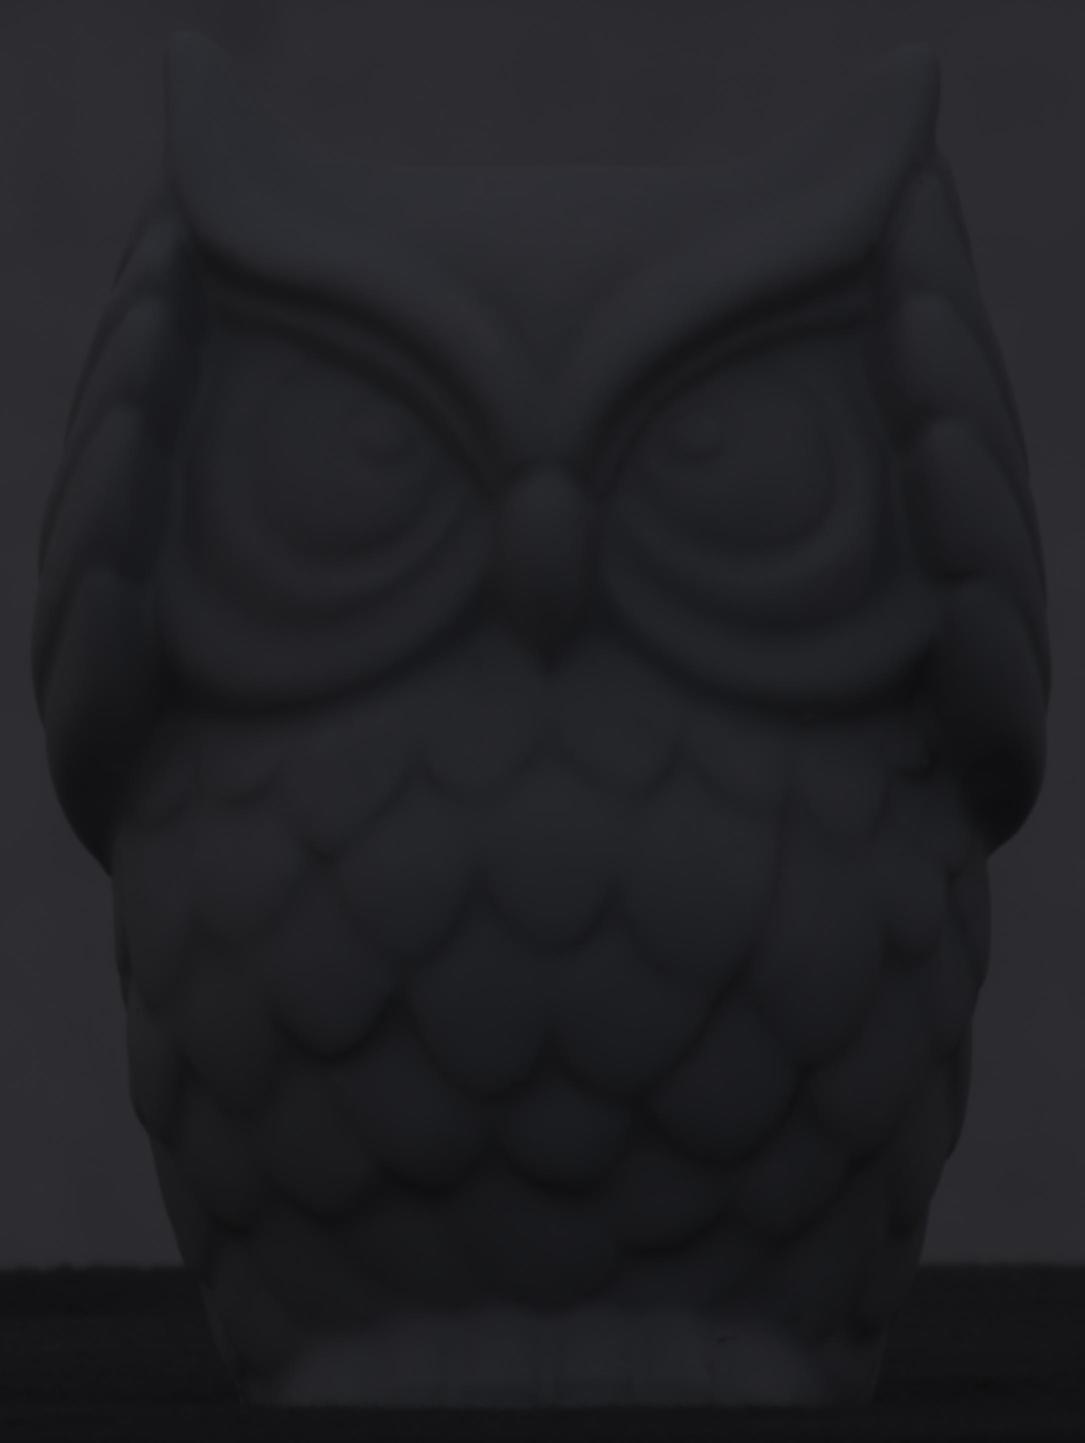
\includegraphics[width=\customwidth]{./figures/reconstruction/object/160215.jpg}

    \end{tabular}
    \caption{Real outdoor HDR images of owl statuette and corresponding HDR environment maps (top row) providing synchronized, high-fidelity estimates of illumination conditions. All images were acquired on 10/11/2014 and tone-mapped for display only (with $\gamma = 1.6$). The sun visibility was 43\% on this day. }
    \label{fig:reconstruction:example_envmaps}
    \vspace{-1em}
\end{figure*}

We oriented this owl statuette towards south and took 66 HDR captures using a Canon EOS Rebel SL1 between 10h30 and 16h30, local time, in Quebec City. These captures were synchronized with the HDR environment maps described in sec.~\ref{sec:hdrdb}, providing high fidelity estimates of the illumination conditions for each image, as shown in fig.~\ref{fig:reconstruction:example_envmaps}. The laser scan was then manually aligned to these images.

A simple outdoor PS algorithm was run on evenly distributed patches on the owl images. For each patch, the surface normal is obtained as to minimize the rendering error given by the model in~\eqref{eqn:matrix-form}, in a least-squares sense. Since this estimation problem is nonlinear on the normal ${\bf n}$, a solution is computed via exhaustive search on a set of 271 candidate orientations for the light hemisphere $\Omega_{\bf n}$. Given $\Omega_{\bf n}$, a candidate solution ${\bf x}$ is obtained via linear least squares. For the best solution, an estimation error, in degrees, is computed using the reference normal from the laser scan. The uncertainty measure (confidence interval $\mathcal{C}_{\bf n}$) derived in sec.~\ref{subsec:measure_uncertainty} is also computed for each patch.

Results from this quantitative evaluation are given in fig.~\ref{fig:reconstruction:results}. As shown on the left, normals pointing upwards are generally recovered more accurately than normals pointing downwards. This is in concordance with the predicted confidence intervals shown on the right in fig.~\ref{fig:reconstruction:results}. The behavior of the reconstruction error is, in general, well predicted by the confidence intervals.
% Note however that the ground truth normals were aligned with the images manually, therefore slight misalignments could explain discrepancies.


\begin{figure}[t]
    \centering
    \newcommand{\customwidthres}{0.45\linewidth}
    \begin{tabular}{cc}
        \scriptsize Angular differences to ground truth & \scriptsize Predicted 95\% confidence intervals \\
        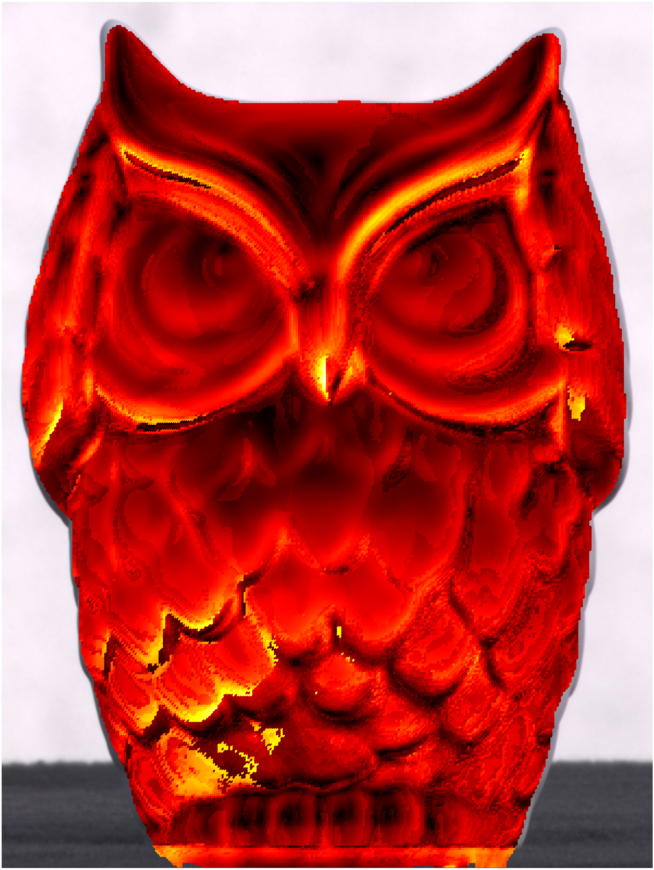
\includegraphics[width=\customwidthres]{./figures/reconstruction/owl_delta_gt.png} &
        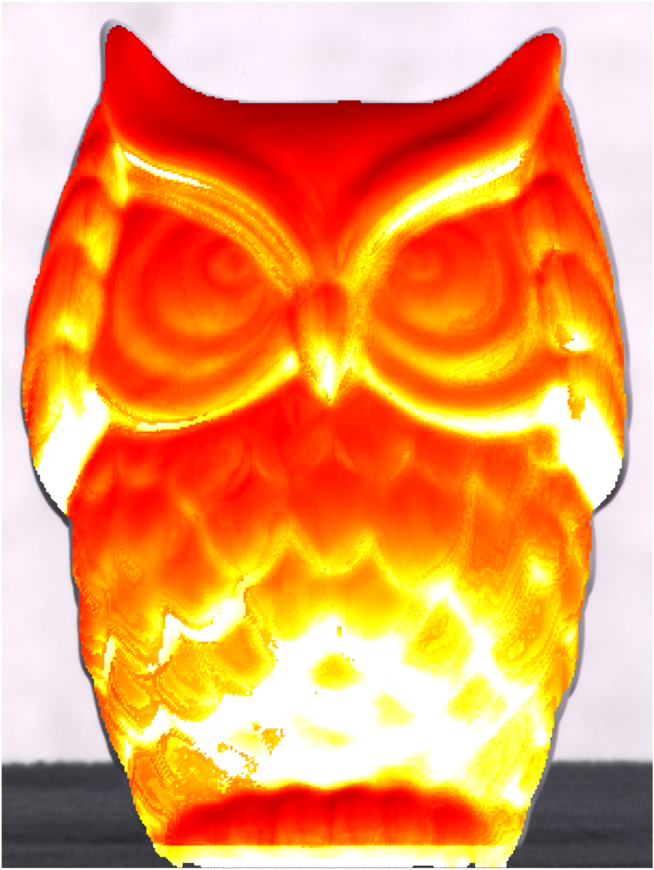
\includegraphics[width=\customwidthres]{./figures/reconstruction/owl_confint.png}
        \begin{picture}(0,0)
            \put(-155,-2){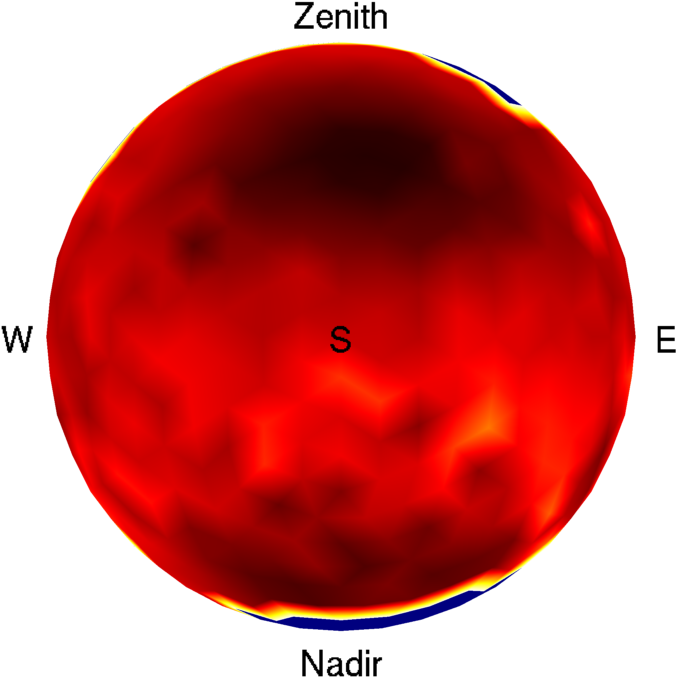
\includegraphics[height=1.5cm]{./figures/reconstruction/owl_sphere_dgt.png}}
            \put(-35,-2){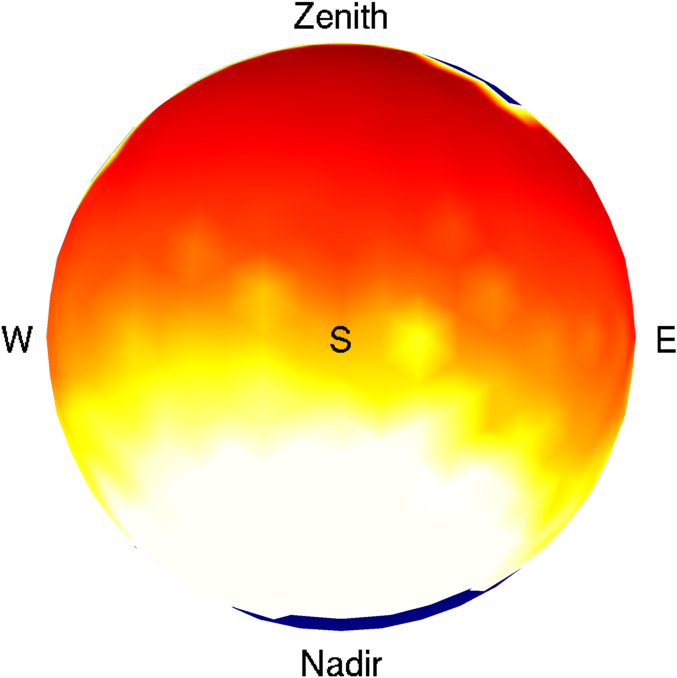
\includegraphics[height=1.5cm]{./figures/reconstruction/owl_sphere_ci.png}}
        \end{picture}
    \end{tabular}
    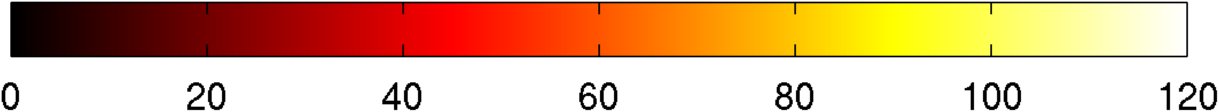
\includegraphics[width=1.01\linewidth]{./figures/reconstruction/colorbar.png}
    \caption{Quantitative validation on images of a real object. Evenly distributed patches of the owl images were used to perform a simple calibrated outdoor PS algorithm. Error estimates of the surface normals are reported on the left using the reference surface orientation in the laser scan. The predicted 95\% confidence intervals $\mathcal{C}_\mathbf{n}$ from \eqref{eqn:confidence-degrees} are shown on the right. A few large estimation errors on the left image may be caused by imperfect alignment between the scanned model and the images. Insets in the lower right corner show the recovered normals mapped to the south hemisphere. Normals in dark blue means no data available.}
    \label{fig:reconstruction:results}
\end{figure}


\subsubsection{Discussion and future work}
\label{sec:iccp-discussion}

This paper has presented the first data-driven analysis of the expected behavior of PS under outdoor illumination. In this scenario, we have no control over the illumination conditions themselves, so existing methods to determine an optimal illumination setup~\cite{drbohlav-iccv-05,klaudiny-prl-14} cannot be applied. Our goal is, therefore, to reveal natural factors that distinguish good and unfavorable daylight conditions for outdoor PS.

The recent work of Shen et al.~\cite{shen-pg-14} presents an insightful, theoretical analysis of the conditioning of outdoor PS using the standard illumination model with a point light source. Their work suggests that PS reconstruction becomes unstable in two cases of nearly planar sun motion: near the poles during the winter solstices, and worldwide near the equinoxes. However, these conclusions are drawn based on a simple illumination model that focuses exclusively on direct sun light, without considering other atmospheric components. Our approach is fundamentally different in that we adopt a more realistic illumination model and then follow a data-driven approach to investigate the conditioning of outdoor PS. We identify not only solar, but also atmospheric and object-intrinsic factors that contribute to stability, or uncertainty, in the photometric reconstruction.

% mention PS in one vs multiple days above?

To achieve our goal, we exploit a large database of outdoor HDR environment maps that provide a rich sampling of the natural variability in outdoor illumination. To make comprehensive use of this dataset, our photometric model considers not only direct sun illumination, but also the full atmospheric (sky) component and an additional ground effect. We then derive a theoretical analysis to investigate the stability of surface normal reconstruction, as measured by an intuitive angular confidence interval. Our empirical analysis reveals how reconstruction is affected by surface orientation, cloud coverage, and sun elevation. Our preliminary quantitative experiments corroborate the predictions with actual reconstruction results.

%There is an interesting relationship between our work and the recent work of Shen et al.~\cite{shen-pg-14}. Their work uses a geometrical analysis to show that, as a function of time of year and latitude, the sun path is sometimes \emph{not} planar and it alone can be used to estimate surface normals reliably. In our case, we employ a data-driven approach which considers the impact of the entire sky hemisphere (including the sun position), the normal direction, camera parameters, and surface reflectance. \todo{Write this when we have more details about the influence of the sun elevation}.

In short, our analysis revealed the following important observations of direct practical value. We show that better stability can be achieved when:
\begin{enumerate}[nosep]
    \item surface patches are oriented South and above the horizon: since our data was captured in the Northern Hemisphere, these are the patches (normals) that ``see'' the sun while it moves during the day;
    \item the sky is partially cloudy throughout the day: this resulted in improved stability than either completely sunny, or completely overcast days;
    \item the sun is lower in the sky: this resulted, on average, in slightly better performance than with days where the sun is higher in the sky.
\end{enumerate}
% In short, our analysis revealed important observations of direct practical value. First, better stability is typically observed for surface patches oriented south and above the horizon. Since our data was captured in the Northern Hemisphere, these are the patches (normals) that ``see'' the sun while it moves during the day. Second, partially cloudy conditions resulted in better stability than either completely sunny, or completely overcast days. Third, days with lower sun elevations yielded, on average, slightly better performance than days with higher sun elevations.
While these observations might seem intuitive to an experienced practitioner, as far as we know, our work is the first attempt to confirm or contradict such intuition in outdoor PS. For instance, a common belief has been that clear days were preferable~\cite{yu-iccp-13,inose-tcva-13,ackermann-cvpr-12,abrams-eccv-12}, instead of mixed weather.

Another goal of this paper has been to inform future research in outdoor PS. Clearly, a better understanding of the sources of uncertainty is useful in developing better reconstruction algorithms (\eg, better informed regularization). Despite the interesting observations above, this work still has some limitations that also open the way to interesting future work. First, it would be interesting to explore the correlation between the predicted reconstruction performance (\eg, fig.~\ref{fig:objects}) and the performance of an actual outdoor photometric stereo algorithm such as~\cite{yu-iccp-13}. Second, our analysis assumes white Gaussian noise, for practical purposes; more realistic noise models for HDR photography should be investigated. Third, our current analysis does not model random perturbations in the light probes themselves (\ie,~${\bf L}$). These are interesting extensions that increase the complexity of our derivations above and, thus, are left as future work. Finally, some seasons are not well represented in our dataset yet. We plan on continuing data capture to further enrich this database of outdoor environment maps.
